% Task C25
% Source volume: lower
% Physical scan pages: 348--382
% Printed book pages: 336--370
% Transcribe only source content; omit running headers, footers, and printed page numbers.
\chapter{曲面积分}

曲面积分与曲线积分一样也有两类：与曲面的方向无关的第一型曲面积分和与曲面的方向有关的第二型曲面积分。本章在 §25.1 和 §25.2 两节中讨论 $\RR^3$ 中的这两类曲面积分以及它们之间的关系，所有的概念和结果都可以推广到 $\RR^n$（$n>3$）的情况。在 §25.3 中介绍 Gauss 公式（第二型曲面积分与三重积分之间的关系），Stokes（斯托克斯）公式（第二型曲面积分与第二型曲线积分之间的关系），以及在 $\RR^3$ 中曲线积分与路径无关的条件。在 §25.4 中介绍一些外微分的初步知识。最后一节是习题课教案一例、学习要点和参考题。

\section{第一型曲面积分}

\subsection{第一型曲面积分的定义和计算}

在 22.5.1 小节中我们在假定曲面面积存在的情况下，推导出了曲面面积的计算公式，下面给出曲面面积的严格定义。考虑一个以分段光滑的闭曲线 $L$ 为边界的光滑曲面 $S$，设这一曲面被一个分段光滑的曲线网分成许多部分 $S_1,S_2,\ldots,S_m$，并在每一部分 $S_i$ 内任取一点 $M_i$，把元素 $S_i$ 垂直地投影到曲面在点 $M_i$ 处的切平面上，得到在切平面内的平面图形 $T_i$，其面积 $\Delta T_i$（$i=1,2,\ldots,m$）的和在各个元素 $S_i$ 的直径趋于零时的极限
\[
  \lim_{\lambda\to0}\sum_i \Delta T_i
\]
称为曲面 $S$ 的面积，其中 $\lambda=\max_{1\le i\le m}\{d(S_i)\}$ 为 $S_i$（$i=1,2,\ldots,m$）中的最大直径。如果极限为有限数，则称曲面 $S$ 为可求面积的。

设 $S$ 是 $\RR^3$ 中的可求面积的曲面，函数 $f$ 在 $S$ 上有定义。对于 $S$ 的任一分割 $T:\{S_1,S_2,\ldots,S_m\}$，用 $\Delta S_i$ 表示 $S_i$ 的面积，任取 $(\xi_i,\eta_i,\zeta_i)\in S_i$，如果当
\[
  d(T)=\max_{1\le i\le m}d(S_i)\to0
\]
时，和数
\[
  \sum_i f(\xi_i,\eta_i,\zeta_i)\Delta S_i
\]
收敛，且极限不依赖于 $S$ 的具体分割与 $(\xi_i,\eta_i,\zeta_i)\in S_i$ 的具体选择，则称函数 $f$ 在 $S$ 上的第一型曲面积分存在，该极限值称为 $f(x,y,z)$ 在 $S$ 上的第一型曲面积分，记为
\[
  \iint_S f(x,y,z)\,\dd S
  =\lim_{d(T)\to0}\sum_i f(\xi_i,\eta_i,\zeta_i)\Delta S_i.
\]

如果曲面 $S$ 的参数方程是
\[
  x=x(u,v),\qquad y=y(u,v),\qquad z=z(u,v),\qquad (u,v)\in D,
\]
$D$ 是 $uOv$ 平面上可求面积的区域，$x(u,v),y(u,v),z(u,v)$ 在 $D$ 上有连续偏导数，则
\[
  \dd S=\sqrt{EG-F^2}\,\dd u\,\dd v,
\]
其中
\[
  E=x_u^2+y_u^2+z_u^2,
  \qquad F=x_ux_v+y_uy_v+z_uz_v,
  \qquad G=x_v^2+y_v^2+z_v^2,
\]
且
\begin{equation}
  \iint_S f(x,y,z)\,\dd S
  =\iint_D f(x(u,v),y(u,v),z(u,v))\sqrt{EG-F^2}\,\dd u\,\dd v.
  \tag{25.1}
\end{equation}
特别地，若曲面 $S$ 的方程为
\[
  z=z(x,y),\qquad (x,y)\in D,
\]
则
\begin{equation}
  \iint_S f(x,y,z)\,\dd S
  =\iint_D f(x,y,z(x,y))\sqrt{1+z_x^2+z_y^2}\,\dd x\,\dd y.
  \tag{25.2}
\end{equation}

\begin{xexample}[25.1.1]
设 $S$ 为 $z=\sqrt{x^2+y^2}$ 被 $x^2+y^2=2ax$ 割下的部分，求
\[
  I=\iint_S (x^2y^2+y^2z^2+z^2x^2)\,\dd S.
\]
\end{xexample}

\begin{xsolution}
\textbf{1}\quad 见图 25.1，在直角坐标系中计算
\[
  z_x=\frac{x}{z},\qquad z_y=\frac{y}{z},
\]
\[
  \sqrt{1+z_x^2+z_y^2}=\sqrt2,
\]
\[
  I=\iint_{x^2+y^2\le2ax}[x^2y^2+(x^2+y^2)^2]\sqrt2\,\dd x\,\dd y.
\]
用极坐标变换求上述二重积分，则
\begin{align*}
I&=\sqrt2\int_{-\pi/2}^{\pi/2}\dd\theta\int_0^{2a\cos\theta}
(r^4\cos^2\theta\sin^2\theta+r^4)r\,\dd r\\
&=\sqrt2\int_{-\pi/2}^{\pi/2}(\cos^2\theta\sin^2\theta+1)
\left.\frac16r^6\right|_0^{2a\cos\theta}\dd\theta\\
&=\frac{\sqrt2}{6}(2a)^6\int_{-\pi/2}^{\pi/2}\cos^6\theta
(\cos^2\theta\sin^2\theta+1)\,\dd\theta
=\frac{29}{8}\sqrt2\pi a^6.
\end{align*}

\begin{center}
  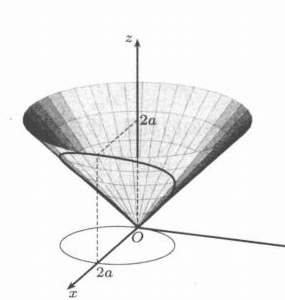
\includegraphics[width=.42\linewidth]{figures/lower/ch25/fig-25-1.png}

  图 25.1
\end{center}

\textbf{2}\quad 用参数式计算。$z=\sqrt{x^2+y^2}$ 在球坐标系中的方程为 $\varphi=\pi/4$，因此 $S$ 的参数方程为
\[
  x=\frac1{\sqrt2}r\cos\theta,\qquad
  y=\frac1{\sqrt2}r\sin\theta,\qquad
  z=\frac1{\sqrt2}r,\qquad (r,\theta)\in D.
\]
又 $S$ 的边界线
\[
  z=\sqrt{x^2+y^2},\qquad x^2+y^2=2ax
\]
的球坐标表示为
\[
  \varphi=\frac\pi4,\qquad r^2\sin^2\varphi=2ar\sin\varphi\cos\theta.
\]
于是
\[
  D=\left\{(r,\theta)\mathrel{\Big|}-\frac\pi2\le\theta\le\frac\pi2,
  \ 0\le r\le2\sqrt2a\cos\theta\right\}.
\]
计算得
\[
  E=\frac{r^2}{2},\qquad F=0,\qquad G=1,
\]
最后得到
\begin{align*}
I&=\int_{-\pi/2}^{\pi/2}\dd\theta\int_0^{2\sqrt2a\cos\theta}
\left(\frac14r^4\cos^2\theta\sin^2\theta+\frac14r^4\right)\frac r{\sqrt2}\,\dd r\\
&=\frac{29}{8}\sqrt2\pi a^6.
\end{align*}
\end{xsolution}

\subsection{第一型曲面积分的应用}

1. 求曲面的面积。在 (25.2) 与 (25.1) 中令 $f=1$，则曲面 $S$ 的面积为
\[
  \iint_S\dd S
  =\iint_{D_{xy}}\sqrt{1+z_x^2+z_y^2}\,\dd x\,\dd y
  =\iint_{D_{uv}}\sqrt{EG-F^2}\,\dd u\,\dd v.
\]

2. 求曲面的质量。设曲面 $S$ 的面密度为 $\rho(x,y,z)$，则它的质量
\[
  m=\iint_S\rho(x,y,z)\,\dd S
  =\iint_D\rho(x(u,v),y(u,v),z(u,v))\sqrt{EG-F^2}\,\dd u\,\dd v.
\]

3. 求曲面的质心坐标。曲面 $S$ 的质心坐标 $(x_0,y_0,z_0)$ 由下面的公式确定：
\[
  x_0=\frac1m\iint_S x\rho(x,y,z)\,\dd S,
\]
\[
  y_0=\frac1m\iint_S y\rho(x,y,z)\,\dd S,
\]
\[
  z_0=\frac1m\iint_S z\rho(x,y,z)\,\dd S.
\]

\begin{xexample}[25.1.2]
求上半球面 $z=\sqrt{a^2-x^2-y^2}$ 被 $x^2+y^2=ax$ 截取部分的面积与质心坐标，其中 $a>0$。
\end{xexample}

\begin{xsolution}
见图 22.11，这就是 Viviani 体的上表面。由于
\[
  z_x=-\frac{x}{\sqrt{a^2-x^2-y^2}},\qquad
  z_y=-\frac{y}{\sqrt{a^2-x^2-y^2}},
\]
故所求面积
\begin{align*}
S&=\iint_{x^2+y^2\le ax}\frac{a}{\sqrt{a^2-x^2-y^2}}\,\dd x\,\dd y\\
&=\int_{-\pi/2}^{\pi/2}\dd\theta\int_0^{a\cos\theta}
\frac{ar}{\sqrt{a^2-r^2}}\,\dd r
=(\pi-2)a^2.
\end{align*}
下面求质心坐标，由对称性知 $y_0=0$，且
\begin{align*}
x_0&=\frac1{(\pi-2)a^2}\iint_S x\,\dd S\\
&=\frac2{(\pi-2)a^2}
\iint_{\substack{x^2+y^2\le ax\\y\ge0}}
\frac{ax}{\sqrt{a^2-x^2-y^2}}\,\dd x\,\dd y\\
&=\frac2{(\pi-2)a}\int_0^{\pi/2}\cos\theta\,\dd\theta
\int_0^{a\cos\theta}\frac{r^2}{\sqrt{a^2-r^2}}\,\dd r
\qquad(r=a\cos t)\\
&=\frac2{(\pi-2)a}\int_0^{\pi/2}\cos\theta\,\dd\theta
\int_{\pi/2}^{\theta}\frac{a^2\cos^2 t}{a\sin t}(-a\sin t)\,\dd t\\
&=\frac a{\pi-2}\int_0^{\pi/2}\cos\theta
\left(\frac\pi2-\theta-\sin\theta\cos\theta\right)\,\dd\theta\\
&=\frac{2a}{3(\pi-2)};
\end{align*}
\begin{align*}
z_0&=\frac1{(\pi-2)a^2}\iint_S z\,\dd S\\
&=\frac1{(\pi-2)a^2}\iint_{x^2+y^2\le ax}
\frac{a}{\sqrt{a^2-x^2-y^2}}\sqrt{a^2-x^2-y^2}\,\dd x\,\dd y\\
&=\frac{\pi a}{4(\pi-2)}.
\end{align*}
\end{xsolution}

\subsection{练习题}

\begin{xexercise}[1]
求 $\iint_S z^2\,\dd S$，其中
\begin{enumerate}[label=(\arabic*)]
\item $S$ 为 $z^2=x^2+y^2$ 在 $x^2+y^2+z^2=R^2$ 内的上半部分（$z\ge0$）；
\item $S$ 为 $x=r\sin\alpha\cos\theta,\ y=r\sin\alpha\sin\theta,\ z=r\cos\alpha$，$0\le r\le a$，$0\le\theta\le2\pi$。
\end{enumerate}
\end{xexercise}
\begin{xsolution}
\textbf{（1）}\quad
在上半锥面上取柱坐标参数
\[
  x=r\cos\theta,\qquad y=r\sin\theta,\qquad z=r,
  \qquad 0\le\theta\le2\pi.
\]
由球面条件
\[
  x^2+y^2+z^2=2r^2\le R^2
\]
知 $0\le r\le R/\sqrt2$。参数曲面的面积元为
\[
  \dd S=\sqrt2\,r\,\dd r\,\dd\theta.
\]
因此
\begin{align*}
\iint_S z^2\,\dd S
&=\sqrt2\int_0^{2\pi}\int_0^{R/\sqrt2}r^3\,\dd r\,\dd\theta\\
&=2\pi\sqrt2\cdot\frac14\left(\frac{R}{\sqrt2}\right)^4
=\frac{\pi\sqrt2}{8}R^4.
\end{align*}

\textbf{（2）}\quad
令
\[
  \vect X(r,\theta)
  =(r\sin\alpha\cos\theta,r\sin\alpha\sin\theta,r\cos\alpha).
\]
则
\[
  \left|\vect X_r\times\vect X_\theta\right|=r\sin\alpha
\]
（按通常球坐标约定 $0\le\alpha\le\pi$；若不作此约定，应写成 $r|\sin\alpha|$）。于是
\begin{align*}
\iint_S z^2\,\dd S
&=\int_0^{2\pi}\int_0^a r^2\cos^2\alpha\,r\sin\alpha\,\dd r\,\dd\theta\\
&=\frac{\pi a^4}{2}\sin\alpha\cos^2\alpha.
\end{align*}
\end{xsolution}


\begin{xexercise}[2]
求 $\iint_S(x+y+z)\,\dd S$，其中 $S$ 为上半单位球面 $x^2+y^2+z^2=1$（$z\ge0$）。
\end{xexercise}
\begin{xsolution}
在上半单位球面上，由关于 $xOz$、$yOz$ 平面的对称性，
\[
  \iint_Sx\,\dd S=\iint_Sy\,\dd S=0.
\]
取球坐标 $z=\cos\varphi$，$0\le\varphi\le\pi/2$，则
\[
  \dd S=\sin\varphi\,\dd\varphi\,\dd\theta.
\]
故
\[
  \iint_S(x+y+z)\,\dd S
  =\int_0^{2\pi}\int_0^{\pi/2}\cos\varphi\sin\varphi\,\dd\varphi\,\dd\theta
  =\pi.
\]
\end{xsolution}


\begin{xexercise}[3]
求 $\iint_S(x+y+z)^2\,\dd S$，其中 $S$ 为单位球面 $x^2+y^2+z^2=1$。
\end{xexercise}
\begin{xsolution}
展开被积函数：
\[
  (x+y+z)^2=x^2+y^2+z^2+2xy+2yz+2zx.
\]
在单位球面上，三个交叉项的积分均由对称性为零，而
\[
  \iint_S(x^2+y^2+z^2)\,\dd S=\iint_S1\,\dd S=4\pi.
\]
所以
\[
  \iint_S(x+y+z)^2\,\dd S=4\pi.
\]
\end{xsolution}


\begin{xexercise}[4]
求 $\iint_S(x^4-y^4+y^2z^2-z^2x^2+1)\,\dd S$，其中 $S$ 是锥面 $z^2=x^2+y^2$ 被柱面 $x^2+y^2=2x$ 割下的部分。
\end{xexercise}
\begin{xsolution}
在锥面 $z^2=x^2+y^2$ 上，
\begin{align*}
&x^4-y^4+y^2z^2-z^2x^2+1\\
&=x^4-y^4+y^2(x^2+y^2)-x^2(x^2+y^2)+1=1.
\end{align*}
柱面 $x^2+y^2=2x$ 在 $xOy$ 平面上的投影是圆盘
\[
  (x-1)^2+y^2\le1,
\]
面积为 $\pi$。锥面的上、下两叶均满足 $\dd S=\sqrt2\,\dd x\,\dd y$，故
\[
  \iint_S\dd S=2\sqrt2\,\pi.
\]
因此原积分为
\[
  \boxed{2\sqrt2\pi}.
\]
\end{xsolution}


\begin{xexercise}[5]
求 $\iint_S|xyz|\,\dd S$，其中
\begin{enumerate}[label=(\arabic*)]
\item $S$ 为 $|x|+|y|+|z|=1$；
\item $S$ 是抛物面 $z=x^2+y^2$ 被 $z=1$ 割下的部分。
\end{enumerate}
\end{xexercise}
\begin{xsolution}
\textbf{（1）}\quad
由对称性，只需计算第一卦限内的三角形面
\[
  z=1-x-y,\qquad x\ge0,\ y\ge0,\ x+y\le1,
\]
再乘以 $8$。该面上 $\dd S=\sqrt3\,\dd x\,\dd y$，故
\begin{align*}
\iint_S|xyz|\,\dd S
&=8\sqrt3\int_0^1\int_0^{1-x}xy(1-x-y)\,\dd y\,\dd x\\
&=8\sqrt3\cdot\frac1{120}
=\frac{\sqrt3}{15}.
\end{align*}

\textbf{（2）}\quad
令
\[
  x=r\cos\theta,\qquad y=r\sin\theta,\qquad z=r^2,
  \qquad 0\le r\le1,\ 0\le\theta\le2\pi.
\]
则
\[
  \dd S=r\sqrt{1+4r^2}\,\dd r\,\dd\theta,
\]
且
\[
  |xyz|=r^4|\cos\theta\sin\theta|.
\]
利用
\[
  \int_0^{2\pi}|\cos\theta\sin\theta|\,\dd\theta=2,
\]
得到
\[
  I=2\int_0^1r^5\sqrt{1+4r^2}\,\dd r.
\]
令 $u=1+4r^2$，则
\begin{align*}
I
&=\frac1{64}\int_1^5(u-1)^2u^{1/2}\,\dd u\\
&=\frac1{64}\left[\frac27u^{7/2}-\frac45u^{5/2}+\frac23u^{3/2}\right]_1^5\\
&=\frac{125\sqrt5-1}{420}.
\end{align*}
\end{xsolution}


\begin{xexercise}[6]
求 $\iint_S(x^2+y^2+z^2)\,\dd S$，$S$ 为 $|x|+|y|+|z|=a$。
\end{xexercise}
\begin{xsolution}
设 $a>0$。由八面对称性，在第一卦限只需计算
\[
  z=a-x-y,\qquad x\ge0,\ y\ge0,\ x+y\le a,
\]
其面积元为 $\sqrt3\,\dd x\,\dd y$。由单纯形积分
\[
  \int_0^a\int_0^{a-x}x^2\,\dd y\,\dd x
  =\frac{a^4}{12},
\]
而 $x^2,y^2,z^2$ 的积分相同，故第一卦限一个面的积分为
\[
  \sqrt3\cdot3\frac{a^4}{12}=\frac{\sqrt3}{4}a^4.
\]
乘以 $8$ 得
\[
  \boxed{2\sqrt3\,a^4}.
\]
\end{xsolution}


\begin{xexercise}[7]
求
\[
  F(t)=\iint_{x^2+y^2+z^2=t^2}f(x,y,z)\,\dd S,
\]
其中
\[
  f(x,y,z)=
  \begin{cases}
    x^2+y^2,& z\ge\sqrt{x^2+y^2},\\
    0,& z<\sqrt{x^2+y^2}.
  \end{cases}
\]
\end{xexercise}
\begin{xsolution}
球面半径为 $|t|$。被积函数非零的部分满足
\[
  z\ge\sqrt{x^2+y^2},
\]
即球坐标中的 $0\le\varphi\le\pi/4$。在该球冠上
\[
  x^2+y^2=t^2\sin^2\varphi,\qquad
  \dd S=t^2\sin\varphi\,\dd\varphi\,\dd\theta.
\]
所以
\begin{align*}
F(t)
&=2\pi t^4\int_0^{\pi/4}\sin^3\varphi\,\dd\varphi\\
&=2\pi t^4\left(\frac23-\frac{5\sqrt2}{12}\right)\\
&=\frac{\pi}{6}(8-5\sqrt2)t^4.
\end{align*}
$t=0$ 时右端也为 $0$，故此式对所有实数 $t$ 均成立。
\end{xsolution}


\begin{xexercise}[8]
求 $F(x,y,z,t)=\iint_S f(\xi,\eta,\zeta)\,\dd S$，其中 $S$ 为
\[
  (x-\xi)^2+(y-\eta)^2+(z-\zeta)^2=t^2,
\]
$t>0$，$(x,y,z)$ 为满足 $\sqrt{x^2+y^2+z^2}>a>0$ 的定点，
\[
  f(\xi,\eta,\zeta)=
  \begin{cases}
  1,& \xi^2+\eta^2+\zeta^2<a^2,\\
  0,& \xi^2+\eta^2+\zeta^2\ge a^2.
  \end{cases}
\]
\end{xexercise}
\begin{xsolution}
记
\[
  d=\sqrt{x^2+y^2+z^2}>a.
\]
所求积分就是以定点 $(x,y,z)$ 为球心、半径为 $t$ 的球面落在球 $\xi^2+\eta^2+\zeta^2<a^2$ 内的面积。

若 $t\le d-a$ 或 $t\ge d+a$，两球面没有形成正面积的相交球冠，故 $F=0$。若
\[
  d-a<t<d+a,
\]
取球面上从球心指向原点的方向为极轴，记极角为 $\theta$。球面上一点到原点的距离平方为
\[
  d^2+t^2-2dt\cos\theta.
\]
条件小于 $a^2$ 等价于
\[
  \cos\theta>\frac{d^2+t^2-a^2}{2dt}=:c.
\]
因此相交部分是球冠，其面积为
\[
  2\pi t^2(1-c)
  =\frac{\pi t}{d}\bigl[a^2-(d-t)^2\bigr].
\]
故
\[
F(x,y,z,t)=
\begin{cases}
\dfrac{\pi t}{d}\bigl[a^2-(d-t)^2\bigr],&d-a<t<d+a,\\[5pt]
0,&0<t\le d-a\text{ 或 }t\ge d+a.
\end{cases}
\]
在相切情形边界圆面积为零，上式的分段取值一致。
\end{xsolution}


\begin{xexercise}[9]
求 $\iint_S\dfrac{\dd S}{(1+x+y)^2}$，其中 $S$ 为立体 $x+y+z\le1,\ x\ge0,\ y\ge0,\ z\ge0$ 的表面。
\end{xexercise}
\begin{xsolution}
立体是第一卦限中的四面体，其表面由 $x=0,y=0,z=0$ 与 $x+y+z=1$ 四个面组成。

在 $x=0$ 面上，
\begin{align*}
I_x
&=\int_0^1\int_0^{1-y}\frac{\dd z\,\dd y}{(1+y)^2}
=\int_0^1\frac{1-y}{(1+y)^2}\,\dd y
=1-\ln2.
\end{align*}
在 $y=0$ 面上同样直接积分：
\[
I_y=\int_0^1\int_0^{1-x}\frac{\dd z\,\dd x}{(1+x)^2}
=\int_0^1\frac{1-x}{(1+x)^2}\,\dd x
=1-\ln2.
\]

在 $z=0$ 面上，以 $s=x+y$ 分层可得
\[
I_z=\int_0^1\frac{s}{(1+s)^2}\,\dd s
=\ln2-\frac12.
\]
斜面 $z=1-x-y$ 的面积元为 $\sqrt3\,\dd x\,\dd y$，故
\[
I_{\text{斜面}}=\sqrt3\left(\ln2-\frac12\right).
\]
相加得到
\[
  \boxed{\frac{3-\sqrt3}{2}+(\sqrt3-1)\ln2}.
\]
\end{xsolution}


\begin{xexercise}[10]
求 $\iint_S\dfrac{|x|}{z}\,\dd S$，其中 $S$ 是柱面 $x^2+y^2=2ay$ 被锥面 $z=\sqrt{x^2+y^2}$ 和平面 $z=2a$ 所截下的部分。
\end{xexercise}
\begin{xsolution}
柱面的柱线在 $xOy$ 平面上的极坐标方程为
\[
  r=2a\sin\theta,\qquad0\le\theta\le\pi.
\]
取参数
\[
  x=2a\sin\theta\cos\theta,\qquad
  y=2a\sin^2\theta,\qquad
  2a\sin\theta\le z\le2a.
\]
平面圆周的弧长元为 $2a\,\dd\theta$，所以柱面面积元为
\[
  \dd S=2a\,\dd\theta\,\dd z.
\]
于是
\begin{align*}
I
&=2a^2\int_0^\pi|\sin2\theta|
   \int_{2a\sin\theta}^{2a}\frac{\dd z}{z}\,\dd\theta\\
&=2a^2\int_0^\pi|\sin2\theta|[-\ln(\sin\theta)]\,\dd\theta.
\end{align*}
由关于 $\pi/2$ 的对称性，
\begin{align*}
\int_0^\pi|\sin2\theta|[-\ln(\sin\theta)]\,\dd\theta
&=2\int_0^{\pi/2}\sin2\theta[-\ln(\sin\theta)]\,\dd\theta\\
&=\int_0^1-\ln u\,\dd u=1,
\end{align*}
其中令 $u=\sin^2\theta$。故
\[
  \boxed{I=2a^2}.
\]
\end{xsolution}


\begin{xexercise}[11]
求 $\iint_S(x^2+y^2)\,\dd S$，$S$ 是锥面 $z=\sqrt{x^2+y^2}$ 被 $z=1$ 割下的部分。
\end{xexercise}
\begin{xsolution}
在锥面 $z=\sqrt{x^2+y^2}=r$ 上，$0\le r\le1$，且
\[
  \dd S=\sqrt2\,r\,\dd r\,\dd\theta.
\]
因此
\[
  \iint_S(x^2+y^2)\,\dd S
  =\sqrt2\int_0^{2\pi}\int_0^1r^3\,\dd r\,\dd\theta
  =\frac{\pi\sqrt2}{2}.
\]
\end{xsolution}


\section{第二型曲面积分}

\subsection{第二型曲面积分的定义和计算}

设 $S$ 是逐片光滑的定向曲面，$P,Q,R$ 是在曲面 $S$ 上有定义的函数。在曲面 $S$ 所指定的一侧作分割 $T$，它把曲面 $S$ 分为 $n$ 个小曲面 $S_1,S_2,\ldots,S_n$，分割 $T$ 的细度
\[
  \|T\|=\max_{1\le i\le n}\{S_i\text{ 的直径}\}.
\]
以 $\Delta S_i^{(1)},\Delta S_i^{(2)},\Delta S_i^{(3)}$ 分别表示 $S_i$ 在 $yOz,xOz,xOy$ 三个坐标平面上的投影区域的面积，它们的符号由 $S_i$ 的方向来确定，当 $S_i$ 的法线正向与 $z$ 轴正向成锐角时，$S_i$ 在 $xOy$ 平面的投影区域的面积 $\Delta S_i^{(3)}$ 为正，反之面积为负。$\Delta S_i^{(1)}$ 与 $\Delta S_i^{(2)}$ 的符号可类似地定义。在每个 $S_i$ 上任取一点 $(\xi_i,\eta_i,\zeta_i)$，若
\begin{align*}
&\lim_{\|T\|\to0}\sum_{i=1}^nP(\xi_i,\eta_i,\zeta_i)\Delta S_i^{(1)}
+\lim_{\|T\|\to0}\sum_{i=1}^nQ(\xi_i,\eta_i,\zeta_i)\Delta S_i^{(2)}\\
&\qquad+\lim_{\|T\|\to0}\sum_{i=1}^nR(\xi_i,\eta_i,\zeta_i)\Delta S_i^{(3)}
\end{align*}
存在，且与曲面 $S$ 的分割 $T$ 以及 $(\xi_i,\eta_i,\zeta_i)$ 在 $S_i$ 上的取法无关，则称此极限为函数 $P,Q,R$ 在曲面 $S$ 上所指定的一侧上的第二型曲面积分，记为
\[
  \iint_S P(x,y,z)\,\dd y\,\dd z+Q(x,y,z)\,\dd z\,\dd x+R(x,y,z)\,\dd x\,\dd y.
\]

设 $R(x,y,z)$ 是定义在光滑曲面
\[
  S:z=z(x,y),\qquad (x,y)\in D_{xy}
\]
上的连续函数，以 $S$ 的上侧为正侧，则有
\[
  \iint_S R(x,y,z)\,\dd x\,\dd y
  =\pm\iint_{D_{xy}}R(x,y,z(x,y))\,\dd x\,\dd y.
\]
如果在正侧积分，积分号前取正号；如果在负侧积分，积分号前取负号。

类似地，当 $P(x,y,z)$ 在光滑曲面
\[
  S:x=x(y,z),\qquad (y,z)\in D_{yz}
\]
上连续时，有
\[
  \iint_S P(x,y,z)\,\dd y\,\dd z
  =\pm\iint_{D_{yz}}P(x(y,z),y,z)\,\dd y\,\dd z,
\]
这里 $S$ 是以 $S$ 的法线方向与 $x$ 轴的正向成锐角的那一侧为正侧。

当 $Q(x,y,z)$ 在光滑曲面
\[
  S:y=y(z,x),\qquad (z,x)\in D_{zx}
\]
上连续时，有
\[
  \iint_S Q(x,y,z)\,\dd z\,\dd x
  =\pm\iint_{D_{zx}}Q(x,y(z,x),z)\,\dd z\,\dd x,
\]
这里 $S$ 是以 $S$ 的法线方向与 $y$ 轴的正向成锐角的那一侧为正侧。

如果光滑曲面 $S$ 由参数方程给出：
\[
  S:x=x(u,v),\quad y=y(u,v),\quad z=z(u,v),\quad (u,v)\in D,
\]
且行列式
\[
  A=\frac{\partial(y,z)}{\partial(u,v)},\qquad
  B=\frac{\partial(z,x)}{\partial(u,v)},\qquad
  C=\frac{\partial(x,y)}{\partial(u,v)}
\]
不同时为 0，则
\begin{equation}
  \iint_S P\,\dd y\,\dd z+Q\,\dd z\,\dd x+R\,\dd x\,\dd y
  =\pm\iint_D(PA+QB+RC)\,\dd u\,\dd v.
  \tag{25.3}
\end{equation}
其中积分号前正负号的选取法则如下：若向量 $(A,B,C)$ 与曲面 $S$ 上预先选定的侧的法向量方向所成角不大于直角，则取“$+$”号，否则取“$-$”号。

\begin{xexample}[25.2.1]
设 $\Sigma$ 为上半单位球面 $z=\sqrt{1-(x^2+y^2)}$，取内侧，求
\[
  I=\iint_\Sigma \dd y\,\dd z+\dd z\,\dd x+\dd x\,\dd y.
\]
\end{xexample}

\begin{xsolution}
\textbf{1}\quad 用直角坐标系计算
\[
  I=\iint_\Sigma\dd y\,\dd z+\iint_\Sigma\dd z\,\dd x+\iint_\Sigma\dd x\,\dd y=I_1+I_2+I_3.
\]
计算 $I_1$：$\Sigma=\Sigma_1+\Sigma_2$，其中
\[
  \Sigma_1:x=\sqrt{1-y^2-z^2},\quad (y,z)\in D_{yz}=\{y^2+z^2\le1,z\ge0\},\quad\text{取后侧},
\]
\[
  \Sigma_2:x=-\sqrt{1-y^2-z^2},\quad (y,z)\in D_{yz},\quad\text{取前侧},
\]
则
\[
  I_1=\iint_{\Sigma_1}\dd y\,\dd z+\iint_{\Sigma_2}\dd y\,\dd z
  =-\iint_{D_{yz}}\dd y\,\dd z+\iint_{D_{yz}}\dd y\,\dd z=0.
\]
同理有
\[
  I_2=0,\qquad I_3=-\iint_{D_{xy}}\dd x\,\dd y=-\pi.
\]
最后得到 $I=-\pi$。

\textbf{2}\quad 用参数方程
\[
  \Sigma:x=\sin\varphi\cos\theta,\quad y=\sin\varphi\sin\theta,\quad z=\cos\varphi,
\]
\[
  0\le\varphi\le\frac\pi2,\qquad 0\le\theta\le2\pi.
\]
计算行列式
\[
  A=\frac{\partial(y,z)}{\partial(\varphi,\theta)}=\sin^2\varphi\cos\theta,
  \quad
  B=\frac{\partial(z,x)}{\partial(\varphi,\theta)}=\sin^2\varphi\sin\theta,
\]
\[
  C=\frac{\partial(x,y)}{\partial(\varphi,\theta)}=\sin\varphi\cos\varphi.
\]
因为 $(A,B,C)$ 的方向与上半球面 $S$ 内侧的法线方向相反，故积分号前取“$-$”号，得到
\begin{align*}
I&=-\iint_D(\sin^2\varphi\cos\theta+\sin^2\varphi\sin\theta+\sin\varphi\cos\varphi)\,\dd\varphi\,\dd\theta\\
&=-\int_0^{\pi/2}\dd\varphi\int_0^{2\pi}
[\sin^2\varphi(\cos\theta+\sin\theta)+\sin\varphi\cos\varphi]\,\dd\theta\\
&=-2\pi\int_0^{\pi/2}\sin\varphi\cos\varphi\,\dd\varphi=-\pi.
\end{align*}
\end{xsolution}

\begin{xexample}[25.2.2]
求
\[
  I=\oiint_\Sigma(z+x)\,\dd y\,\dd z+(x+y)\,\dd z\,\dd x+(y+z)\,\dd x\,\dd y,
\]
其中 $\Sigma$ 是由 $x^2+y^2=1$、$z=1$ 及三个坐标平面围成的立体在第一卦限的部分的表面，取外侧。
\end{xexample}

\begin{center}
  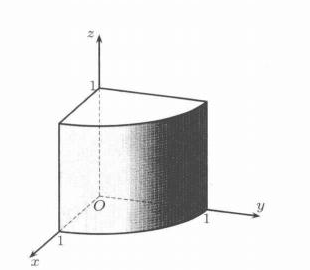
\includegraphics[width=.36\linewidth]{figures/lower/ch25/fig-25-2.png}

  图 25.2
\end{center}

\begin{xsolution}
见图 25.2，因为 $\Sigma$ 分块较多（需分 5 块），不便于用参数式，故应在直角坐标系中计算。记 $\Sigma=\Sigma_1+\Sigma_2+\Sigma_3+\Sigma_4+\Sigma_5$，其中 $\Sigma_1$ 为圆柱面，$\Sigma_2$ 为下底面，$\Sigma_3$ 为上底面，$\Sigma_4$ 为左侧面 $y=0$，$\Sigma_5$ 为右侧面 $x=0$，则有
\[
  I=\oiint_\Sigma(z+x)\,\dd y\,\dd z+
  \oiint_\Sigma(x+y)\,\dd z\,\dd x+
  \oiint_\Sigma(y+z)\,\dd x\,\dd y=I_1+I_2+I_3.
\]
计算 $I_1$，有
\[
  I_1=\sum_{i=1}^5\iint_{\Sigma_i}(x+z)\,\dd y\,\dd z.
\]
因为 $\Sigma_2,\Sigma_3,\Sigma_4$ 在 $yOz$ 平面上的投影面积为零，于是
\[
  \iint_{\Sigma_i}(x+z)\,\dd y\,\dd z=0,\qquad i=2,3,4,
\]
而
\[
  \Sigma_1:x=\sqrt{1-y^2},\quad(y,z)\in D_{yz}=\{0\le y\le1,0\le z\le1\},\quad\text{取前侧},
\]
\[
  \Sigma_5:x=0,\quad(y,z)\in D_{yz},\quad\text{取后侧}.
\]
于是
\begin{align*}
I_1&=\iint_{\Sigma_1}(x+z)\,\dd y\,\dd z+\iint_{\Sigma_5}(x+z)\,\dd y\,\dd z\\
&=\iint_{D_{yz}}(\sqrt{1-y^2}+z)\,\dd y\,\dd z-
\iint_{D_{yz}}z\,\dd y\,\dd z\\
&=\int_0^1\int_0^1\sqrt{1-y^2}\,\dd y\,\dd z=\frac\pi4.
\end{align*}
用类似的方法可求出 $I_2=\pi/4$。然后求
\[
  I_3=\sum_{i=1}^5\iint_{\Sigma_i}(y+z)\,\dd x\,\dd y.
\]
显然有
\[
  \iint_{\Sigma_i}(y+z)\,\dd x\,\dd y=0,\qquad i=1,4,5,
\]
而
\[
  \Sigma_2:z=0,\quad(x,y)\in D_{xy}=\{x^2+y^2\le1,x\ge0,y\ge0\},\quad\text{取下侧},
\]
\[
  \Sigma_3:z=1,\quad(x,y)\in D_{xy},\quad\text{取上侧},
\]
于是
\begin{align*}
I_3&=\iint_{\Sigma_2}(y+z)\,\dd x\,\dd y+\iint_{\Sigma_3}(y+z)\,\dd x\,\dd y\\
&=-\iint_{D_{xy}}y\,\dd x\,\dd y+\iint_{D_{xy}}(1+y)\,\dd x\,\dd y\\
&=\iint_{D_{xy}}\dd x\,\dd y=\frac\pi4.
\end{align*}
最后得到
\[
  I=I_1+I_2+I_3=\frac34\pi.
\]
\end{xsolution}

\begin{xremark}
我们已经知道，利用第二型曲线积分可以计算平面图形的面积。类似地，利用第二型曲面积分也可以计算空间立体的体积（见表达式 (25.7)--(25.11)）。
\end{xremark}

\subsection{两类曲面积分之间的关系}

设 $S$ 是可定向曲面，$\vect n$ 是 $S$ 上选定的某一侧的法向量，则
\begin{equation}
\begin{aligned}
&\iint_S P\,\dd y\,\dd z+Q\,\dd z\,\dd x+R\,\dd x\,\dd y\\
&\qquad=\iint_S[P\cos(\vect n,x)+Q\cos(\vect n,y)+R\cos(\vect n,z)]\,\dd S.
\end{aligned}
\tag{25.4}
\end{equation}
上述关系式的用处之一是可简化曲面积分的计算，当某一类曲面积分的计算比较复杂时，可利用公式 (25.4) 转化为另一类曲面积分进行计算。

\begin{xexample}[25.2.3]
求
\[
  I=\iint_\Sigma xyz(y^2z^2+z^2x^2+x^2y^2)\,\dd S,
\]
其中 $\Sigma$ 为第一卦限中的球面 $x^2+y^2+z^2=a^2$（$x\ge0,y\ge0,z\ge0$）。
\end{xexample}

\begin{xsolution}
见图 25.3，不论用参数式或直角坐标式，直接计算均相当复杂。取 $\Sigma$ 的上侧，则 $(x,y,z)$ 处的单位外法向量为 $(x/a,y/a,z/a)$，利用公式 (25.4)，
\begin{align*}
I&=a\iint_\Sigma\left(y^3z^3\frac xa+z^3x^3\frac ya+x^3y^3\frac za\right)\,\dd S\\
&=a\iint_\Sigma y^3z^3\,\dd y\,\dd z+z^3x^3\,\dd z\,\dd x+x^3y^3\,\dd x\,\dd y\\
&=3a\iint_\Sigma x^3y^3\,\dd x\,\dd y
=3a\iint_{D_{xy}}x^3y^3\,\dd x\,\dd y,
\end{align*}
其中 $D_{xy}=\{x^2+y^2\le a^2,x\ge0,y\ge0\}$，作极坐标变换得
\[
  I=3a\int_0^{\pi/2}\dd\theta\int_0^a r^7\sin^3\theta\cos^3\theta\,\dd r
  =\frac3{64}a^9\int_0^{\pi/2}\sin^3 2\theta\,\dd\theta
  =\frac1{32}a^9.
\]
\end{xsolution}

\begin{center}
  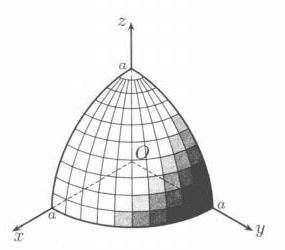
\includegraphics[width=.31\linewidth]{figures/lower/ch25/fig-25-3.png}\qquad
  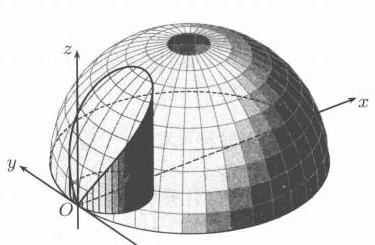
\includegraphics[width=.40\linewidth]{figures/lower/ch25/fig-25-4.png}

  图 25.3\hspace{7em}图 25.4
\end{center}

\begin{xexample}[25.2.4]
求
\[
  I=\iint_\Sigma(y-z)\,\dd y\,\dd z+(z-x)\,\dd z\,\dd x+(x-y)\,\dd x\,\dd y,
\]
其中 $\Sigma$ 是球面 $x^2+y^2+z^2=2Rx$ 被柱面 $x^2+y^2=2rx$（$0<r<R$）截下的位于 $z\ge0$ 的部分，取外侧。
\end{xexample}

\begin{xsolution}
见图 25.4，改写球面方程为 $(x-R)^2+y^2+z^2=R^2$，其外侧的法向量
\[
  \vect n=\left(\frac{x-R}{R},\frac yR,\frac zR\right).
\]
由公式 (25.4)，有
\begin{align*}
I&=\iint_\Sigma(y-z,z-x,x-y)\cdot\vect n\,\dd S\\
&=\frac1R\iint_\Sigma[(y-z)(x-R)+(z-x)y+(x-y)z]\,\dd S\\
&=\iint_\Sigma(z-y)\,\dd S.
\end{align*}
由于 $\Sigma$ 关于 $xOz$ 平面对称，而函数 $y$ 是奇函数，于是
\begin{align*}
I&=\iint_\Sigma z\,\dd S
=\iint_{x^2+y^2\le2rx}\sqrt{2Rx-x^2-y^2}\,
\frac{R}{\sqrt{2Rx-x^2-y^2}}\,\dd x\,\dd y\\
&=R\cdot\pi r^2=\pi Rr^2.
\end{align*}
\end{xsolution}

\subsection{练习题}

\begin{xexercise}[1]
设曲面 $\Sigma$ 的方程为 $z=z(x,y),(x,y)\in D$，且 $z(x,y)$ 在 $\overline D$ 中连续可微，证明：
\[
\begin{aligned}
  &\iint_\Sigma P(x,y,z)\,\dd y\,\dd z
  +Q(x,y,z)\,\dd z\,\dd x\\
  &\qquad+R(x,y,z)\,\dd x\,\dd y\\
  &\quad=\pm\iint_D(-Pz_x-Qz_y+R)\big|_{z=z(x,y)}\,\dd x\,\dd y.
\end{aligned}
\]
当 $\Sigma$ 取上侧时符号取“$+$”；当 $\Sigma$ 取下侧时符号取“$-$”。
\end{xexercise}
\begin{xsolution}
用 $(x,y)$ 作为参数，
\[
  \vect X(x,y)=(x,y,z(x,y)).
\]
公式 (25.3) 中三个行列式为
\[
A=\frac{\partial(y,z)}{\partial(x,y)}=-z_x,
\qquad
B=\frac{\partial(z,x)}{\partial(x,y)}=-z_y,
\qquad
C=\frac{\partial(x,y)}{\partial(x,y)}=1.
\]
代入 (25.3) 即得
\[
  \iint_\Sigma P\,\dd y\,\dd z+Q\,\dd z\,\dd x+R\,\dd x\,\dd y
  =\pm\iint_D(-Pz_x-Qz_y+R)\big|_{z=z(x,y)}\,\dd x\,\dd y.
\]
参数面积向量 $(-z_x,-z_y,1)$ 的第三分量为正，指向曲面的上侧，所以 $\Sigma$ 取上侧时取“$+$”，取下侧时取“$-$”。
\end{xsolution}


\begin{xexercise}[2]
若 $\Sigma$ 分块光滑，且关于 $xOy$ 平面对称，$f(x,y,z)$ 在 $\Sigma$ 上连续，且满足 $f(x,y,z)=-f(x,y,-z)$，问：
\[
  \iint_\Sigma f(x,y,z)\,\dd S=2\iint_{\Sigma_1}f(x,y,z)\,\dd S
\]
还是等于 $0$？（其中 $\Sigma_1$ 是 $\Sigma$ 在 $xOy$ 平面以上的部分。）
\end{xexercise}
\begin{xsolution}
把 $\Sigma$ 分成上、下两部分 $\Sigma_1,\Sigma_2$。映射
\[
  T(x,y,z)=(x,y,-z)
\]
把 $\Sigma_1$ 等面积地映到 $\Sigma_2$，即 $\dd S$ 不变。又由条件
\[
  f(x,y,-z)=-f(x,y,z),
\]
故
\[
  \iint_{\Sigma_2}f\,\dd S=-\iint_{\Sigma_1}f\,\dd S.
\]
因此
\[
  \boxed{\iint_\Sigma f\,\dd S=0}.
\]
\end{xsolution}


\begin{xexercise}[3]
若 $\Sigma$ 分块光滑，且关于 $xOy$ 平面对称，$R(x,y,z)$ 在 $\Sigma$ 上连续，满足 $R(x,y,z)=-R(x,y,-z)$，问：
\[
  \iint_\Sigma R(x,y,z)\,\dd x\,\dd y=2\iint_{\Sigma_1}R(x,y,z)\,\dd x\,\dd y
\]
还是等于 $0$？（其中 $\Sigma_1$ 是 $\Sigma$ 在 $xOy$ 平面以上的部分，取侧与 $\Sigma$ 取侧相一致。）
\end{xexercise}
\begin{xsolution}
把第二型积分写成第一型积分：
\[
  \iint_\Sigma R\,\dd x\,\dd y
  =\iint_\Sigma R\cos(\vect n,z)\,\dd S.
\]
在关于 $xOy$ 平面的反射下，取侧相一致意味着法向量的第三分量变号，因此
\[
  \cos(\vect n,z)(x,y,-z)=-\cos(\vect n,z)(x,y,z).
\]
同时 $R$ 也是关于 $z$ 的奇函数，所以乘积
\[
  R\cos(\vect n,z)
\]
在上下两部分取相同的值。故
\[
  \boxed{
  \iint_\Sigma R\,\dd x\,\dd y
  =2\iint_{\Sigma_1}R\,\dd x\,\dd y}.
\]
\end{xsolution}


\begin{xexercise}[4]
设 $\Sigma$ 是平面 $\Pi$ 内的一个有界区域，其面积为 $S$，$\Pi$ 取上侧的法向量为 $\vect n$，且 $\cos(\vect n,z)=\mu$，证明：$\Sigma$ 在 $xOy$ 平面上的投影的面积为 $\mu S$，并利用这个结果重新计算例题 21.4.2。
\end{xexercise}
\begin{xsolution}
平面 $\Pi$ 上单位法向量 $\vect n$ 为常向量，且
\[
  \cos(\vect n,z)=\mu.
\]
平面面积元与其在 $xOy$ 平面的有向投影面积元满足
\[
  \dd x\,\dd y=\cos(\vect n,z)\,\dd S=\mu\,\dd S.
\]
由于题中取的是上侧，$\mu\ge0$。对 $\Sigma$ 积分即得其投影面积
\[
  S_{xy}=\iint_\Sigma\mu\,\dd S=\mu S.
\]

对例题 21.4.2，椭圆在 $xOy$ 平面上的投影区域满足
\[
  \frac{x^2}{3}+y^2+\frac{(2x+y)^2}{2}\le1,
\]
即
\[
  14x^2+12xy+9y^2\le6.
\]
二次型矩阵
\[
  \begin{pmatrix}14&6\\6&9\end{pmatrix}
\]
的特征值为 $5,18$，故经正交变换后投影椭圆可写成
\[
  5u^2+18v^2\le6.
\]
因此其面积为
\[
  S_{xy}=\pi\sqrt{\frac65}\sqrt{\frac13}
  =\frac{\sqrt{10}}5\pi.
\]
例题中平面的单位法向量与 $z$ 轴正向夹角的余弦为
\[
  \mu=\frac1{\sqrt6},
\]
于是所求椭圆面积为
\[
  \boxed{S=\frac{S_{xy}}\mu=\frac{2\sqrt{15}}5\pi}.
\]
\end{xsolution}


\begin{xexercise}[5]
求 $I_1=\iint_\Sigma z\,\dd x\,\dd y$，$I_2=\iint_\Sigma z^2\,\dd x\,\dd y$，$\Sigma$ 是球面 $x^2+y^2+z^2=a^2$，取外侧。
\end{xexercise}
\begin{xsolution}
球面取外侧。由 Gauss 公式，
\[
  I_1=\oiint_\Sigma z\,\dd x\,\dd y
  =\iiint_{x^2+y^2+z^2\le a^2}1\,\dd x\,\dd y\,\dd z
  =\frac{4\pi a^3}{3}.
\]
对第二个积分再次应用 Gauss 公式：
\[
  I_2=\oiint_\Sigma z^2\,\dd x\,\dd y
  =\iiint_{x^2+y^2+z^2\le a^2}2z\,\dd x\,\dd y\,\dd z=0.
\]
最后一步由积分区域关于 $xOy$ 平面对称且被积函数 $2z$ 为奇函数得到。因此
\[
  \boxed{I_1=\frac{4\pi a^3}{3},\qquad I_2=0}.
\]
\end{xsolution}


\begin{xexercise}[6]
计算
\[
  \iint_S xz\,\dd y\,\dd z+yz\,\dd z\,\dd x+yz\,\dd x\,\dd y,
\]
$S$ 是圆柱面 $x^2+y^2=1$ 在 $-1\le z\le1$ 及 $x\ge0$ 的部分，取前侧。
\end{xexercise}
\begin{xsolution}
% chapters/ch25.tex 此题第二项误录为 $yz\,\dd z\,\dd x$；原书题面为 $yx\,\dd z\,\dd x$，以下按原书题面计算。
取参数
\[
  x=\cos\theta,\qquad y=\sin\theta,\qquad
  -\frac\pi2\le\theta\le\frac\pi2,\quad -1\le z\le1.
\]
“前侧”对应 $x$ 分量为正的外法向量
\[
  \vect n=(\cos\theta,\sin\theta,0),
\]
且 $\dd S=\dd\theta\,\dd z$。原书题面的三个系数为
\[
  \vect F=(xz,xy,yz).
\]
于是
\begin{align*}
I
&=\iint_S\vect F\cdot\vect n\,\dd S\\
&=\int_{-\pi/2}^{\pi/2}\int_{-1}^{1}
  \bigl(z\cos^2\theta+\cos\theta\sin^2\theta\bigr)
  \,\dd z\,\dd\theta.
\end{align*}
第一项关于 $z$ 为奇函数，积分为零；第二项与 $z$ 无关，因此
\begin{align*}
I
&=2\int_{-\pi/2}^{\pi/2}\cos\theta\sin^2\theta\,\dd\theta
=\frac43.
\end{align*}
故
\[
  \boxed{I=\frac43}.
\]
\end{xsolution}


\begin{xexercise}[7]
求
\[
  \iint_S x(z^2-y^2)\,\dd y\,\dd z+y(x^2-z^2)\,\dd z\,\dd x+z(y^2-x^2)\,\dd x\,\dd y,
\]
其中 $S$ 是 $y^2+z^2=1$ 被 $x=0,x=1,z+y=0,z-y=0$ 截取的上方部分，取外侧。
\end{xexercise}
\begin{xsolution}
圆柱轴为 $x$ 轴。取
\[
  y=\sin\theta,\qquad z=\cos\theta,\qquad
  -\frac\pi4\le\theta\le\frac\pi4,\qquad0\le x\le1,
\]
这正对应被 $z+y=0$、$z-y=0$ 截出的上方部分。外法向量为
\[
  \vect n=(0,y,z),
\]
且 $\dd S=\dd x\,\dd\theta$。令
\[
\vect F=\bigl(x(z^2-y^2),\ y(x^2-z^2),\ z(y^2-x^2)\bigr).
\]
则
\[
  \vect F\cdot\vect n=x^2(y^2-z^2)=-x^2\cos2\theta.
\]
因此
\begin{align*}
I
&=-\int_0^1x^2\,\dd x\int_{-\pi/4}^{\pi/4}\cos2\theta\,\dd\theta
=-\frac13.
\end{align*}
\end{xsolution}


\section{Gauss 公式与 Stokes 公式}

\subsection{Gauss 公式}

Gauss 公式是将 $\RR^3$ 中某区域上的三重积分与这一区域的边界上特定的曲面积分建立联系的一个重要公式。

设 $D$ 是 $\RR^3$ 内的一个有界区域，其边界 $\partial D$ 由光滑曲面或逐片光滑曲面组成，方向是外侧（相对于区域 $D$ 而言）。又设函数 $P,Q,R$ 都在 $D$ 上有关于 $x,y,z$ 的连续偏导数，则成立下列 Gauss 公式：
\begin{equation}
  \iiint_D\left(\frac{\partial P}{\partial x}+\frac{\partial Q}{\partial y}+\frac{\partial R}{\partial z}\right)
  \,\dd x\,\dd y\,\dd z
  =\oiint_{\partial D}P\,\dd y\,\dd z+Q\,\dd z\,\dd x+R\,\dd x\,\dd y.
  \tag{25.5}
\end{equation}
利用两类曲面积分之间的关系，Gauss 公式也可以写成
\begin{equation}
\begin{aligned}
  \iiint_D\left(\frac{\partial P}{\partial x}+\frac{\partial Q}{\partial y}+\frac{\partial R}{\partial z}\right)
  \,\dd x\,\dd y\,\dd z
  =\oiint_{\partial D}[P\cos(\vect n,x)+Q\cos(\vect n,y)+R\cos(\vect n,z)]\,\dd S,
\end{aligned}
\tag{25.6}
\end{equation}
其中 $\vect n$ 为曲面 $\partial D$ 上的外法向量。

可以看出，Green 公式 (24.9) 与 Gauss 公式 (25.6) 的表达形式是类似的，仅仅是空间的维数不同而已。

与 Green 公式相仿，Gauss 公式 (25.5) 与 (25.6) 为我们提供了一种新的计算曲面积分的方法。

\begin{xexample}[25.3.1]
求
\[
  I=\iint_\Sigma 4xz\,\dd y\,\dd z-2yz\,\dd z\,\dd x+(1-z^2)\,\dd x\,\dd y,
\]
其中 $\Sigma$ 是曲线 $z=\ee^y$（$0\le y\le a$）绕 $z$ 轴旋转生成的旋转面，取下侧。
\end{xexample}

\begin{xsolution}
$\Sigma$ 的方程为
\[
  z=\ee^{\sqrt{x^2+y^2}}\qquad(x^2+y^2\le a^2).
\]

\begin{center}
  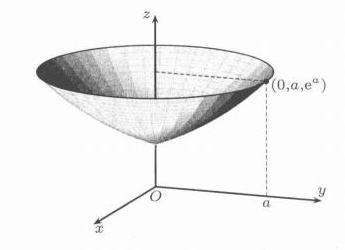
\includegraphics[width=.36\linewidth]{figures/lower/ch25/fig-25-5.png}

  图 25.5
\end{center}

直接计算比较复杂，考虑用 Gauss 公式。由于 $\Sigma$ 不闭，需要添加辅助面
\[
  \Sigma_1:z=\ee^a\quad(x^2+y^2\le a^2),\quad\text{取上侧}.
\]
见图 25.5，设 $\Sigma$ 与 $\Sigma_1$ 围成的区域为 $D$。令
\[
  P=4xz,\qquad Q=-2yz,\qquad R=1-z^2,
\]
则
\[
  \frac{\partial P}{\partial x}+\frac{\partial Q}{\partial y}+\frac{\partial R}{\partial z}=0.
\]
由公式 (25.5)，得
\begin{align*}
I&=\left(\iiint_D+\iint_{\Sigma_1}-\iint_{\Sigma_1}\right)(1-z^2)\,\dd x\,\dd y\\
&=-\iint_{\Sigma_1}(1-z^2)\,\dd x\,\dd y\\
&=(\ee^{2a}-1)\iint_{x^2+y^2\le a^2}\dd x\,\dd y
=(\ee^{2a}-1)\pi a^2.
\end{align*}
\end{xsolution}

\begin{xexample}[25.3.2]
计算曲面积分
\[
  I=\iint_S\frac{x\,\dd y\,\dd z+y\,\dd z\,\dd x+z\,\dd x\,\dd y}{(ax^2+by^2+cz^2)^{3/2}},
\]
其中 $S$ 是球面 $x^2+y^2+z^2=1$，取外侧（$a>0,b>0,c>0$）。
\end{xexample}

\begin{xsolution}
\textbf{1}\quad 记
\[
P(x,y,z)=\frac{x}{(ax^2+by^2+cz^2)^{3/2}},\quad
Q(x,y,z)=\frac{y}{(ax^2+by^2+cz^2)^{3/2}},
\]
\[
R(x,y,z)=\frac{z}{(ax^2+by^2+cz^2)^{3/2}},
\]
则在不包含原点的任何区域上
\[
  \frac{\partial P}{\partial x}+\frac{\partial Q}{\partial y}+\frac{\partial R}{\partial z}=0.
\]
为了利用 Gauss 公式，对充分小的 $\varepsilon>0$，作闭曲面
\[
  S_\varepsilon=\{ax^2+by^2+cz^2=\varepsilon^2\},
\]
取外侧。由 Gauss 公式
\[
  I=\oiint_{S_\varepsilon}\frac{x\,\dd y\,\dd z+y\,\dd z\,\dd x+z\,\dd x\,\dd y}{(ax^2+by^2+cz^2)^{3/2}}
  =\frac1{\varepsilon^3}\oiint_{S_\varepsilon}x\,\dd y\,\dd z+y\,\dd z\,\dd x+z\,\dd x\,\dd y.
\]
上述积分在 $S_\varepsilon$ 的外侧。再一次用 Gauss 公式，则
\[
  I=\frac3{\varepsilon^3}\iiint_{ax^2+by^2+cz^2\le\varepsilon^2}\dd x\,\dd y\,\dd z
  =\frac3{\varepsilon^3}\cdot\frac{4\pi}{3}\cdot\frac{\varepsilon^3}{\sqrt{abc}}
  =\frac{4\pi}{\sqrt{abc}}.
\]

\textbf{2（不用 Gauss 公式而直接计算）}\quad 利用单位球面的参数方程
\[
  x=\sin\varphi\cos\theta,\qquad y=\sin\varphi\sin\theta,\qquad z=\cos\varphi,
\]
\[
  0\le\varphi\le\pi,\qquad 0\le\theta\le2\pi,
\]
计算得到
\[
  A=\frac{\partial(y,z)}{\partial(\varphi,\theta)}=\sin^2\varphi\cos\theta,
  \quad B=\frac{\partial(z,x)}{\partial(\varphi,\theta)}=\sin^2\varphi\sin\theta,
\]
\[
  C=\frac{\partial(x,y)}{\partial(\varphi,\theta)}=\sin\varphi\cos\varphi.
\]
容易看出，$(A,B,C)$ 的方向与单位球面外侧法线方向相同，故积分号前取“$+$”号，由 (25.3) 得
\[
  I=8\int_0^{\pi/2}\int_0^{\pi/2}
  \frac{\sin\varphi\,\dd\varphi\,\dd\theta}
  {(a\sin^2\varphi\cos^2\theta+b\sin^2\varphi\sin^2\theta+c\cos^2\varphi)^{3/2}}.
\]
先计算对 $\varphi$ 的积分，我们令 $\cos\varphi=t$，则
\begin{align*}
&\int_0^{\pi/2}\frac{\sin\varphi\,\dd\varphi}
{(a\sin^2\varphi\cos^2\theta+b\sin^2\varphi\sin^2\theta+c\cos^2\varphi)^{3/2}}\\
&=\int_0^1\frac{\dd t}{[(a\cos^2\theta+b\sin^2\theta)-(a\cos^2\theta+b\sin^2\theta-c)t^2]^{3/2}}\\
&=\frac1{a\cos^2\theta+b\sin^2\theta}
\left.\frac{t}{[(a\cos^2\theta+b\sin^2\theta)-(a\cos^2\theta+b\sin^2\theta-c)t^2]^{1/2}}\right|_{t=0}^{t=1}\\
&=\frac1{\sqrt c}\cdot\frac1{a\cos^2\theta+b\sin^2\theta}.
\end{align*}
最后得到
\begin{align*}
I&=\frac8{\sqrt c}\int_0^{\pi/2}\frac{\dd\theta}{a\cos^2\theta+b\sin^2\theta}
=\frac8{\sqrt c}\int_0^{+\infty}\frac{\dd t}{a+bt^2}\qquad(t=\tan\theta)\\
&=\frac8{\sqrt c}\frac1{\sqrt{ab}}
\left.\arctan\left(\sqrt{\frac ba}t\right)\right|_0^{+\infty}
=\frac{4\pi}{\sqrt{abc}}.
\end{align*}
\end{xsolution}

\begin{xremark}
利用 Gauss 公式来计算曲面积分在很多情况下是一种有效的手段，但要注意使用 Gauss 公式的条件，要弄清楚在什么情况下要“挖洞”（即用封闭曲面把 $P,Q,R$ 不定义或不可微的点围住）以及选择什么曲面“挖洞”计算更简便。
\end{xremark}

利用 Gauss 公式可导出用曲面积分表示 $\RR^3$ 中具有逐片光滑边界的有界闭区域 $\Omega$ 的体积公式
\begin{equation}
  |\Omega|=\oiint_{\partial\Omega}x\,\dd y\,\dd z
  =\oiint_{\partial\Omega}y\,\dd z\,\dd x
  =\oiint_{\partial\Omega}z\,\dd x\,\dd y
  =\frac13\oiint_{\partial\Omega}x\,\dd y\,\dd z+y\,\dd z\,\dd x+z\,\dd x\,\dd y.
  \tag{25.7}
\end{equation}
上述积分在 $\partial\Omega$ 的外侧进行。由两类曲面积分之间的关系，又有
\begin{equation}
  |\Omega|=\frac13\oiint_{\partial\Omega}(x\cos\alpha+y\cos\beta+z\cos\gamma)\,\dd S,
  \tag{25.8}
\end{equation}
其中 $(\cos\alpha,\cos\beta,\cos\gamma)$ 为 $\partial\Omega$ 的单位外法向量。如果 $\partial\Omega$ 有参数表示
\[
  x=x(u,v),\qquad y=y(u,v),\qquad z=z(u,v),\qquad (u,v)\in D,
\]
则
\begin{equation}
  V=\frac13\left|\iint_D(Ax+By+Cz)\,\dd u\,\dd v\right|,
  \tag{25.9}
\end{equation}
其中
\[
  A=\frac{\partial(y,z)}{\partial(u,v)},\qquad
  B=\frac{\partial(z,x)}{\partial(u,v)},\qquad
  C=\frac{\partial(x,y)}{\partial(u,v)}.
\]
(25.9) 也可以写为
\begin{equation}
  V=\frac13\left|\iint_D
  \begin{vmatrix}
  x&y&z\\x_u&y_u&z_u\\x_v&y_v&z_v
  \end{vmatrix}\,\dd u\,\dd v\right|.
  \tag{25.10}
\end{equation}
特别地，若一个立体的表面在球坐标系中由方程
\[
  r=r(\varphi,\theta),\qquad(\varphi,\theta)\in D
\]
给出，则
\[
  x=r(\varphi,\theta)\sin\varphi\cos\theta,\quad
  y=r(\varphi,\theta)\sin\varphi\sin\theta,\quad
  z=r(\varphi,\theta)\cos\varphi,
\]
代入公式 (25.10) 中得到
\begin{equation}
  V=\frac13\iint_D r^3(\varphi,\theta)\sin\varphi\,\dd\varphi\,\dd\theta.
  \tag{25.11}
\end{equation}
当然，公式 (25.11) 也可以从三重积分中直接得到，事实上
\begin{align*}
V&=\iiint_\Omega\dd x\,\dd y\,\dd z
=\iiint_{\substack{(\varphi,\theta)\in D\\0\le\rho\le r(\varphi,\theta)}}
\rho^2\sin\varphi\,\dd\rho\,\dd\theta\,\dd\varphi\\
&=\iint_D\sin\varphi\,\dd\varphi\,\dd\theta
\int_0^{r(\varphi,\theta)}\rho^2\,\dd\rho
=\frac13\iint_Dr^3(\varphi,\theta)\sin\varphi\,\dd\varphi\,\dd\theta.
\end{align*}

\subsection{练习题}

\begin{xexercise}[1]
利用 Gauss 公式计算积分：
\begin{enumerate}[label=(\arabic*)]
\item $\displaystyle\oiint_S y(x-z)\,\dd y\,\dd z+z^2\,\dd z\,\dd x+(y^2+xz)\,\dd x\,\dd y$，其中 $S$ 是正立方体 $\{(x,y,z)\mid0\le x\le a,0\le y\le a,0\le z\le a\}$（$a>0$）的表面，取内侧；
\item $\displaystyle\oiint_\Sigma(x^3+x)\,\dd y\,\dd z+(y^2-xz)\,\dd z\,\dd x+(z^3+z)\,\dd x\,\dd y$，其中 $\Sigma$ 是球面 $x^2+y^2+z^2=2z$，取外侧；
\item 设 $A_1=x^3-x^2y+z^3,\ A_2=xy^2+y^3,\ A_3=xz+z^2$，$\Sigma$ 是由 $yOz$ 平面上的抛物线 $z=1-y^2$ 与 $z=0$ 所围成的平面区域绕 $z$ 轴旋转后所得的旋转体的表面，取外侧。试求
\[
  \oiint_\Sigma\left(\frac{\partial A_3}{\partial y}-\frac{\partial A_2}{\partial z}\right)\,\dd y\,\dd z
  +\left(\frac{\partial A_1}{\partial z}-\frac{\partial A_3}{\partial x}\right)\,\dd z\,\dd x
  +\left(\frac{\partial A_2}{\partial x}-\frac{\partial A_1}{\partial y}\right)\,\dd x\,\dd y.
\]
\end{enumerate}
\end{xexercise}
\begin{xsolution}
\textbf{（1）}\quad
令
\[
P=y(x-z),\qquad Q=z^2,
\qquad R=y^2+xz.
\]
则
\[
  \frac{\partial P}{\partial x}+\frac{\partial Q}{\partial y}+\frac{\partial R}{\partial z}=x+y.
\]
Gauss 公式给出外侧积分
\[
  \iiint_{[0,a]^3}(x+y)\,\dd x\,\dd y\,\dd z=a^4.
\]
题目取内侧，方向相反，故
\[
  \boxed{I=-a^4}.
\]

\textbf{（2）}\quad
球面可写成
\[
  x^2+y^2+(z-1)^2=1.
\]
令
\[
P=x^3+x,\qquad Q=y^2-xz,\qquad R=z^3+z.
\]
则
\[
  \operatorname{div}\vect F=3x^2+3z^2+2y+2.
\]
记 $w=z-1$。在单位球 $B$ 中，
\[
  \iiint_Bx^2\,\dd V=\iiint_Bw^2\,\dd V=\frac{4\pi}{15},
  \qquad |B|=\frac{4\pi}{3},
\]
且奇函数项积分为零。因此
\[
  \iiint_Bz^2\,\dd V
  =\iiint_B(w+1)^2\,\dd V
  =\frac{4\pi}{15}+\frac{4\pi}{3}=\frac{8\pi}{5}.
\]
由 Gauss 公式
\begin{align*}
I
&=3\frac{4\pi}{15}+3\frac{8\pi}{5}+2\frac{4\pi}{3}
=\frac{124\pi}{15}.
\end{align*}

\textbf{（3）}\quad
题中被积向量正是
\[
  \left(
  \frac{\partial A_3}{\partial y}-\frac{\partial A_2}{\partial z},
  \frac{\partial A_1}{\partial z}-\frac{\partial A_3}{\partial x},
  \frac{\partial A_2}{\partial x}-\frac{\partial A_1}{\partial y}
  \right)=\nabla\times(A_1,A_2,A_3).
\]
由于 $A_1,A_2,A_3$ 是多项式，二阶偏导连续，故
\[
  \operatorname{div}(\nabla\times\vect A)=0.
\]
$\Sigma$ 为闭曲面且取外侧，由 Gauss 公式
\[
  \boxed{I=\iiint_\Omega0\,\dd V=0}.
\]
\end{xsolution}


\begin{xexercise}[2]
先添加辅助面，再用 Gauss 公式计算下列曲面积分：
\begin{enumerate}[label=(\arabic*)]
\item $\displaystyle\iint_\Sigma(x^2\cos\alpha+y^2\cos\beta+z^2\cos\gamma)\,\dd S$，其中 $\Sigma$ 是锥面 $z^2=x^2+y^2$ 在 $0\le z\le h$ 的一段，$(\cos\alpha,\cos\beta,\cos\gamma)$ 为 $\Sigma$ 上的单位法向量，其方向为下方；
\item $\displaystyle\iint_\Sigma x^3\,\dd y\,\dd z+y^3\,\dd z\,\dd x+z^3\,\dd x\,\dd y$，其中 $\Sigma$ 为球面 $x^2+y^2+z^2=a^2$ 之上半部分，取上侧；
\item $\displaystyle\iint_\Sigma\left(\frac{x^3}{a^3}+y^3z^3\right)\,\dd y\,\dd z+
\left(\frac{y^3}{b^3}+z^3x^3\right)\,\dd z\,\dd x+
\left(\frac{z^3}{c^3}+x^3y^3\right)\,\dd x\,\dd y$，其中 $\Sigma$ 为椭球面 $\dfrac{x^2}{a^2}+\dfrac{y^2}{b^2}+\dfrac{z^2}{c^2}=1,\ x\ge0$，取后侧。
\end{enumerate}
\end{xexercise}
\begin{xsolution}
\textbf{（1）}\quad
把锥面与顶面圆盘 $D_h:z=h$ 合起来，围成
\[
  \Omega=\{0\le z\le h,\ x^2+y^2\le z^2\}.
\]
锥面的“下方”法向正是 $\Omega$ 的外法向。令
\[
  \vect F=(x^2,y^2,z^2),
\]
则
\[
  \operatorname{div}\vect F=2(x+y+z).
\]
由旋转对称性，$x,y$ 的体积分为零，所以
\begin{align*}
\iiint_\Omega\operatorname{div}\vect F\,\dd V
&=2\int_0^h z\cdot\pi z^2\,\dd z
=\frac{\pi h^4}{2}.
\end{align*}
顶面取上侧，通量为
\[
  \iint_{D_h}z^2\,\dd x\,\dd y=h^2\cdot\pi h^2=\pi h^4.
\]
故锥面上的所求积分为
\[
  \boxed{-\frac{\pi h^4}{2}}.
\]

\textbf{（2）}\quad
令 $\vect F=(x^3,y^3,z^3)$。在半径为 $a$ 的上半球体中，
\[
  \operatorname{div}\vect F=3(x^2+y^2+z^2)=3r^2.
\]
补上底面 $z=0$；该底面上 $F_z=z^3=0$，没有通量。因此
\begin{align*}
I
&=\iiint_{B_a^+}3r^2\,\dd V
=\frac12\int_0^a3r^2\cdot4\pi r^2\,\dd r
=\frac{6\pi a^5}{5}.
\end{align*}

\textbf{（3）}\quad
设 $\Omega$ 为椭球内部的 $x\ge0$ 一半。题目取“后侧”，即法向量的 $x$ 分量为负，因而与椭球外法向相反。

令
\[
\vect F=\left(\frac{x^3}{a^3}+y^3z^3,
\frac{y^3}{b^3}+z^3x^3,
\frac{z^3}{c^3}+x^3y^3\right).
\]
则
\[
  \operatorname{div}\vect F
  =3\left(\frac{x^2}{a^3}+\frac{y^2}{b^3}+\frac{z^2}{c^3}\right).
\]
补上的平面 $x=0$ 上，外法向为 $(-1,0,0)$，而 $P=y^3z^3$ 的积分由对称性为零。因此椭球半面外侧通量等于上述散度的体积分。

作变换
\[
  x=au,\qquad y=bv,\qquad z=cw.
\]
在半单位球 $u\ge0$ 中
\[
  \iiint u^2\,\dd u\,\dd v\,\dd w
  =\iiint v^2\,\dd u\,\dd v\,\dd w
  =\iiint w^2\,\dd u\,\dd v\,\dd w
  =\frac{2\pi}{15}.
\]
所以外侧通量为
\[
  \frac{2\pi}{5}(bc+ca+ab).
\]
题目方向与此外侧相反，故
\[
  \boxed{I=-\frac{2\pi}{5}(ab+bc+ca)}.
\]
\end{xsolution}


\begin{xexercise}[3]
$F(x,y,z)$ 是定义在 $\RR^3$ 上的光滑函数，且 $F(x,y,z)=0$ 是一个以原点为顶点的锥面 $\Sigma$，如果 $\Sigma$ 与平面 $\Pi:Ax+By+Cz=D$ 围成一个锥体，证明：此锥体的体积
\[
  V=\frac13SH,
\]
其中 $S$ 为平面 $\Pi$ 上锥底部分的面积，$H$ 为顶点到锥底的高。
\end{xexercise}
\begin{xsolution}
记锥体为 $\Omega$，锥底为 $G\subset\Pi$，锥侧为 $\Sigma$。对向量场
\[
  \vect F=(x,y,z)
\]
有 $\operatorname{div}\vect F=3$，故 Gauss 公式给出
\[
  3V=\oiint_{\partial\Omega}\vect F\cdot\vect n\,\dd S.
\]
由于 $F(x,y,z)=0$ 所定义的是以原点为顶点的锥面，锥侧上的每条母线都是从原点出发的射线，因此位置向量 $(x,y,z)$ 沿锥侧切向，故
\[
  \vect F\cdot\vect n=0\qquad\text{在 }\Sigma\text{ 上}.
\]
在锥底平面 $G$ 上，外单位法向量为常向量 $\vect n_0$，而原点到平面的距离为 $H$，于是
\[
  (x,y,z)\cdot\vect n_0=H
\]
（选择外法向后右端取正）。所以
\[
  3V=\iint_GH\,\dd S=HS,
\]
即
\[
  \boxed{V=\frac13SH}.
\]
\end{xsolution}


\begin{xexercise}[4]
求由曲面 $(x^2+y^2+z^2)^2=a^2xy$ 所围成的立体的体积。
\end{xexercise}
\begin{xsolution}
用球坐标
\[
  x=\rho\sin\varphi\cos\theta,
  \quad y=\rho\sin\varphi\sin\theta,
  \quad z=\rho\cos\varphi.
\]
边界方程化为
\[
  \rho^2=a^2\sin^2\varphi\cos\theta\sin\theta.
\]
只有 $\cos\theta\sin\theta\ge0$ 的方向有非零半径，即第一、第三象限方向。于是径向上界为
\[
  \rho_{\max}=a\sin\varphi\sqrt{\cos\theta\sin\theta}.
\]
由球坐标体积公式
\begin{align*}
V
&=\frac{a^3}{3}
\int_0^\pi\sin^4\varphi\,\dd\varphi
\left(2\int_0^{\pi/2}(\sin\theta\cos\theta)^{3/2}\,\dd\theta\right)\\
&=\frac{a^3\pi}{8}B\left(\frac54,\frac54\right).
\end{align*}
利用
\[
  B\left(\frac54,\frac54\right)
  =\frac{\Gamma(5/4)^2}{\Gamma(5/2)}
  =\frac{\Gamma(1/4)^2}{12\sqrt\pi},
\]
得到
\[
  \boxed{V=\frac{a^3\sqrt\pi\,\Gamma(1/4)^2}{96}}.
\]
\end{xsolution}


\begin{xexercise}[5]
求
\[
  \iint_\Sigma(x^3+y^3)\,\dd y\,\dd z+(x^3+2x^2y)\,\dd z\,\dd x-x^2z\,\dd x\,\dd y,
\]
其中 $\Sigma$ 是单叶双曲面 $x^2+y^2-z^2=1$ 在 $0\le z\le\sqrt3$ 的部分，取外侧。
\end{xexercise}
\begin{xsolution}
令
\[
P=x^3+y^3,\qquad Q=x^3+2x^2y,\qquad R=-x^2z.
\]
则
\[
  \operatorname{div}\vect F=3x^2+2x^2-x^2=4x^2.
\]
用 $z=0$ 与 $z=\sqrt3$ 两圆盘封闭双曲面侧面。区域的水平截面满足
\[
  x^2+y^2\le1+z^2.
\]
半径为 $R_0$ 的圆盘上
\[
  \iint x^2\,\dd x\,\dd y=\frac{\pi R_0^4}{4}.
\]
故闭曲面的总外通量为
\begin{align*}
\iiint_\Omega4x^2\,\dd V
&=\pi\int_0^{\sqrt3}(1+z^2)^2\,\dd z\\
&=\frac{24\pi\sqrt3}{5}.
\end{align*}
下底面 $z=0$ 的通量为零；上底面 $z=\sqrt3$ 上
\[
  \iint R\,\dd x\,\dd y
  =-\sqrt3\iint_{x^2+y^2\le4}x^2\,\dd x\,\dd y
  =-4\pi\sqrt3.
\]
所以题目所给双曲面侧面的外侧积分为
\[
  \boxed{\frac{24\pi\sqrt3}{5}+4\pi\sqrt3
  =\frac{44\pi\sqrt3}{5}}.
\]
\end{xsolution}


\begin{xexercise}[6]
$V=\{(x,y,z)\mid x^2+y^2<z<1\}$，$S=\partial V$，求积分
\[
  \oiint_S yz\,\dd z\,\dd x+(x^2+y^2)z\,\dd x\,\dd y,
\]
积分沿外法线方向。
\end{xexercise}
\begin{xsolution}
令
\[
  P=0,\qquad Q=yz,\qquad R=(x^2+y^2)z.
\]
则
\[
  \operatorname{div}\vect F=z+x^2+y^2.
\]
用柱坐标 $r^2=x^2+y^2$，区域为
\[
  0\le r\le1,\qquad r^2<z<1.
\]
由 Gauss 公式
\begin{align*}
I
&=2\pi\int_0^1r\,\dd r\int_{r^2}^{1}(z+r^2)\,\dd z\\
&=2\pi\int_0^1r\left(\frac12+r^2-\frac32r^4\right)\,\dd r
=\frac\pi2.
\end{align*}
\end{xsolution}


\begin{xexercise}[7]
求第二型曲面积分
\[
  \oiint_S z\,\dd y\,\dd z+\cos y\,\dd z\,\dd x+\dd x\,\dd y,
\]
其中 $S$ 为 $x^2+y^2+z^2=1$ 的外侧。
\end{xexercise}
\begin{xsolution}
令
\[
  P=z,\qquad Q=\cos y,\qquad R=1.
\]
则
\[
  \operatorname{div}\vect F=-\sin y.
\]
单位球关于 $y=0$ 平面对称，而 $-\sin y$ 为奇函数，故由 Gauss 公式
\[
  \boxed{I=\iiint_{x^2+y^2+z^2\le1}(-\sin y)\,\dd V=0}.
\]
\end{xsolution}


\subsection{Stokes 公式}

Stokes 公式是将空间曲面上的第二型曲面积分与该曲面边界上的第二型曲线积分之间建立联系的一个重要公式。

设 $D$ 是 $\RR^3$ 中的分片光滑曲面，$D$ 的边界 $\partial D$ 由分段光滑曲线组成，又设 $P,Q,R$ 有关于 $x,y,z$ 的连续偏导数，则成立下列 Stokes 公式：
\begin{equation}
  \oint_{\partial D}P\,\dd x+Q\,\dd y+R\,\dd z
  =\iint_D
  \begin{vmatrix}
  \dd y\,\dd z&\dd z\,\dd x&\dd x\,\dd y\\
  \dfrac\partial{\partial x}&\dfrac\partial{\partial y}&\dfrac\partial{\partial z}\\
  P&Q&R
  \end{vmatrix}.
  \tag{25.12}
\end{equation}
其中 $\partial D$ 的方向和 $D$ 的方向服从右手法则。由两类曲面积分之间的关系 (25.4)，(25.12) 又可以写为
\begin{equation}
  \oint_{\partial D}P\,\dd x+Q\,\dd y+R\,\dd z
  =\iint_D
  \begin{vmatrix}
  \cos\alpha&\cos\beta&\cos\gamma\\
  \dfrac\partial{\partial x}&\dfrac\partial{\partial y}&\dfrac\partial{\partial z}\\
  P&Q&R
  \end{vmatrix}\,\dd S,
  \tag{25.13}
\end{equation}
其中 $\cos\alpha,\cos\beta,\cos\gamma$ 是曲面 $D$ 上法向量的方向余弦。如果曲面 $D$ 在 $xOy$ 平面上，则公式 (25.12)、(25.13) 就是 Green 公式。公式 (25.12) 与 (25.13) 给我们提供了一个求曲线积分与曲面积分的新方法。

\begin{xexample}[25.3.3]
求
\[
  I=\oint_C(y^2-z^2)\,\dd x+(z^2-x^2)\,\dd y+(x^2-y^2)\,\dd z,
\]
其中 $C$ 是立方体 $\{(x,y,z)\mid0\le x\le a,0\le y\le a,0\le z\le a\}$ 的表面与平面 $x+y+z=\frac32a$ 的交线，取向从 $z$ 轴正向看去是逆时针方向。
\end{xexample}

\paragraph{分析}
见图 25.6，分六段积分的计算量很大，且 $C$ 也不便于表示为一个统一的参数式。因 $C$ 为闭曲线，且 $P=y^2-z^2,Q=z^2-x^2,R=x^2-y^2$ 连续可微，故考虑用 Stokes 公式。

\begin{xsolution}
令 $\Sigma$ 为 $x+y+z=\frac32a$ 被 $C$ 所围的一块，取上侧，则 $C$ 的取向与 $\Sigma$ 的取侧相容。应用 Stokes 公式 (25.13)，
\begin{align*}
I&=\iint_\Sigma
\begin{vmatrix}
1/\sqrt3&1/\sqrt3&1/\sqrt3\\
\dfrac\partial{\partial x}&\dfrac\partial{\partial y}&\dfrac\partial{\partial z}\\
y^2-z^2&z^2-x^2&x^2-y^2
\end{vmatrix}\,\dd S\\
&=-\frac1{\sqrt3}\iint_\Sigma4(x+y+z)\,\dd S
=-\frac4{\sqrt3}\iint_\Sigma\frac32a\,\dd S\\
&=-2\sqrt3a\,|\Sigma|=-2\sqrt3a\cdot\frac{3\sqrt3}{4}a^2=-\frac92a^3.
\end{align*}
\end{xsolution}

\begin{center}
  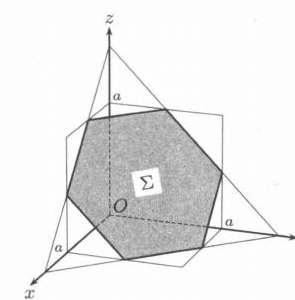
\includegraphics[width=.36\linewidth]{figures/lower/ch25/fig-25-6.png}

  图 25.6
\end{center}

\begin{xexample}[25.3.4]
设 $\Sigma$ 是分片光滑的闭曲面，$\vect n$ 为 $\Sigma$ 上的单位外法向量，证明：
\[
  I=\oiint_\Sigma
  \begin{vmatrix}
  \cos(\vect n,x)&\cos(\vect n,y)&\cos(\vect n,z)\\
  \dfrac\partial{\partial x}&\dfrac\partial{\partial y}&\dfrac\partial{\partial z}\\
  P&Q&R
  \end{vmatrix}\,\dd S=0,
\]
其中分两种情形：（1）$P,Q,R$ 在 $\overline\Omega$ 上二阶连续可微，$\Omega$ 为 $\Sigma$ 所围的立体；（2）$P,Q,R$ 在 $\Sigma$ 上一阶连续可微。
\end{xexample}

\begin{xproof}
对情形（1）用 Gauss 公式
\begin{align*}
I&=\oiint_\Sigma\left(\frac{\partial R}{\partial y}-\frac{\partial Q}{\partial z}\right)\,\dd y\,\dd z
+\left(\frac{\partial P}{\partial z}-\frac{\partial R}{\partial x}\right)\,\dd z\,\dd x\\
&\qquad+\left(\frac{\partial Q}{\partial x}-\frac{\partial P}{\partial y}\right)\,\dd x\,\dd y\\
&=\iiint_\Omega\left[
\frac\partial{\partial x}\left(\frac{\partial R}{\partial y}-\frac{\partial Q}{\partial z}\right)
+\frac\partial{\partial y}\left(\frac{\partial P}{\partial z}-\frac{\partial R}{\partial x}\right)
+\frac\partial{\partial z}\left(\frac{\partial Q}{\partial x}-\frac{\partial P}{\partial y}\right)
\right]\,\dd x\,\dd y\,\dd z=0.
\end{align*}

情形（2）参见图 25.7。在 $\Sigma$ 上任取一条逐段光滑的闭曲线 $C$，$C$ 分 $\Sigma$ 为两部分 $\Sigma_1$ 与 $\Sigma_2$，在 $\Sigma_1,\Sigma_2$ 上分别应用 Stokes 公式，则对于 $i=1,2$，
\[
  \iint_{\Sigma_i}
  \begin{vmatrix}
  \cos(\vect n,x)&\cos(\vect n,y)&\cos(\vect n,z)\\
  \dfrac\partial{\partial x}&\dfrac\partial{\partial y}&\dfrac\partial{\partial z}\\
  P&Q&R
  \end{vmatrix}\,\dd S
  =\oint_{C_i}P\,\dd x+Q\,\dd y+R\,\dd z.
\]
因 $\Sigma_1,\Sigma_2$ 分居 $C$ 两侧，故 $C_1,C_2$ 为同一条曲线 $C$，只是它们的定向相反。若记 $C_1$ 为 $C_+$，则 $C_2$ 为 $C_-$，从而
\[
\begin{aligned}
  I&=\left(\iint_{\Sigma_1}+\iint_{\Sigma_2}\right)
  \begin{vmatrix}
  \cos(\vect n,x)&\cos(\vect n,y)&\cos(\vect n,z)\\
  \dfrac\partial{\partial x}&\dfrac\partial{\partial y}&\dfrac\partial{\partial z}\\
  P&Q&R
  \end{vmatrix}\,\dd S\\
  &=\left(\oint_{C_+}+\oint_{C_-}\right)
  \left(P\,\dd x+Q\,\dd y+R\,\dd z\right)=0.
\end{aligned}
\]
\end{xproof}

\begin{center}
  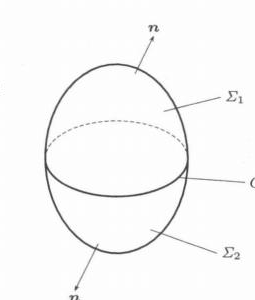
\includegraphics[width=.30\linewidth]{figures/lower/ch25/fig-25-7.png}

  图 25.7
\end{center}

\begin{xexample}[25.3.5]
试用 Stokes 公式计算
\[
  I=\oint_C(y^2+z^2)\,\dd x+(z^2+x^2)\,\dd y+(x^2+y^2)\,\dd z,
\]
其中 $C$ 为 $x^2+y^2+z^2=2Rx$ 与 $x^2+y^2=2rx$ 的交线（$0<r<R,z>0$），$C$ 的定向使得 $C$ 所包围的球面上较小区域保持在左边。
\end{xexample}

\begin{xsolution}
见图 25.4，设 $S$ 为球面 $x^2+y^2+z^2=2Rx$ 被柱面 $x^2+y^2=2rx$ 所截部分的外侧，由 Stokes 公式 (25.13)
\begin{align*}
I&=\iint_S
\begin{vmatrix}
\dfrac{x-R}{R}&\dfrac yR&\dfrac zR\\
\dfrac\partial{\partial x}&\dfrac\partial{\partial y}&\dfrac\partial{\partial z}\\
y^2+z^2&z^2+x^2&x^2+y^2
\end{vmatrix}\,\dd S\\
&=\frac2R\iint_S[(y-z)(x-R)+(z-x)y+(x-y)z]\,\dd S\\
&=2\iint_S(z-y)\,\dd S
=2\iint_S z\,\dd S
=2R\iint_{x^2+y^2\le2rx}\dd x\,\dd y
=2\pi r^2R.
\end{align*}
\end{xsolution}

\subsection{练习题}

\begin{xexercise}[1]
设 $C$ 是平面 $x\cos\alpha+y\cos\beta+z\cos\gamma-\rho=0$ 上逐段光滑的闭曲线，$C$ 所界的面积为 $S$，$C$ 的定向与 $(\cos\alpha,\cos\beta,\cos\gamma)$ 成右手系，试计算积分
\[
  \oint_C
  \begin{vmatrix}
  \dd x&\dd y&\dd z\\
  \cos\alpha&\cos\beta&\cos\gamma\\
  x&y&z
  \end{vmatrix}.
\]
\end{xexercise}
\begin{xsolution}
记
\[
  \vect n=(\cos\alpha,\cos\beta,\cos\gamma),
  \qquad \vect r=(x,y,z).
\]
题中行列式展开后正是
\[
  (\vect n\times\vect r)\cdot\dd\vect r.
\]
令 $\vect F=\vect n\times\vect r$。由于 $\vect n$ 为常单位向量，
\[
  \nabla\times\vect F=2\vect n.
\]
以 $C$ 所围的平面区域为 Stokes 曲面，其单位法向量就是 $\vect n$，所以
\[
  I=\iint_S(2\vect n)\cdot\vect n\,\dd S=2S.
\]
故
\[
  \boxed{I=2S}.
\]
\end{xsolution}


\begin{xexercise}[2]
求 $\oint_C(y-z)\,\dd x+(z-x)\,\dd y+(x-y)\,\dd z$，$C$ 为 $x^2+y^2=1$ 与 $x+y+z=1$ 的交线，从 $x$ 轴正向看是逆时针方向。
\end{xexercise}
\begin{xsolution}
令
\[
  \vect F=(y-z,z-x,x-y).
\]
则
\[
  \nabla\times\vect F=(-2,-2,-2).
\]
取平面
\[
  x+y+z=1
\]
内由 $C$ 围成的圆盘。由于从 $x$ 轴正向看 $C$ 为逆时针，取与之相容的单位法向量
\[
  \vect n=\frac1{\sqrt3}(1,1,1).
\]
该平面圆盘在 $xOy$ 平面的投影是单位圆盘，故其面积为 $\sqrt3\pi$。由 Stokes 公式
\[
  I=(-2,-2,-2)\cdot\frac{(1,1,1)}{\sqrt3}\cdot\sqrt3\pi
  =-6\pi.
\]
\end{xsolution}


\begin{xexercise}[3]
求 $\int_C(z^3+3x^2y)\,\dd x+(x^3+3y^2z)\,\dd y+(y^3+3z^2x)\,\dd z$，其中 $C$ 是 $z=\sqrt{a^2-x^2-y^2}$ 与 $x=y$ 的交线，自 $A(a/\sqrt2,a/\sqrt2,0)$ 到 $B(-a/\sqrt2,-a/\sqrt2,0)$。
\end{xexercise}
\begin{xsolution}
令
\[
P=z^3+3x^2y,\qquad Q=x^3+3y^2z,\qquad R=y^3+3z^2x.
\]
直接计算有
\[
  \nabla\times(P,Q,R)=0.
\]
事实上可取势函数
\[
  \Phi(x,y,z)=xz^3+x^3y+y^3z,
\]
因为 $\dd\Phi=P\,\dd x+Q\,\dd y+R\,\dd z$。所以积分只由端点决定。两端点
\[
A=\left(\frac a{\sqrt2},\frac a{\sqrt2},0\right),
\qquad
B=\left(-\frac a{\sqrt2},-\frac a{\sqrt2},0\right)
\]
均满足
\[
  \Phi(A)=\Phi(B)=\frac{a^4}{4}.
\]
故
\[
  \boxed{\int_C P\,\dd x+Q\,\dd y+R\,\dd z=0}.
\]
\end{xsolution}


\begin{xexercise}[4]
用 Stokes 公式求
\[
  \int_C\ee^{x+z}\{[(x+1)y^2+1]\,\dd x+2xy\,\dd y+xy^2\,\dd z\},
\]
其中 $C$ 是右半柱面 $|x|+|y|=a$（$y>0$）与平面 $y=z$ 的交线从 $(-a,0,0)$ 到 $(a,0,0)$ 的一段（$a>0$）。
\end{xexercise}
\begin{xsolution}
令
\[
\begin{aligned}
P&=\ee^{x+z}([(x+1)y^2+1]),\\
Q&=2xy\ee^{x+z},\\
R&=xy^2\ee^{x+z}.
\end{aligned}
\]
则
\[
  \nabla\times\vect F=(0,\ee^{x+z},0).
\]
原路径 $C$ 位于平面 $y=z$，从
\[
  A=(-a,0,0)
\]
经 $(0,a,a)$ 到
\[
  B=(a,0,0).
\]
补上线段 $L$（从 $B$ 沿 $x$ 轴回到 $A$），得到闭曲线 $C+L$。取三角形
\[
  D=\{(x,y,y)\mid y\ge0,\ |x|+y\le a\}
\]
作为 Stokes 曲面。边界方向 $A\to(0,a,a)\to B\to A$ 对应单位法向量
\[
  \vect n=\frac1{\sqrt2}(0,1,-1).
\]
因此
\begin{align*}
\int_{C+L}\vect F\cdot\dd\vect r
&=\iint_D\ee^{x+y}\,\dd x\,\dd y\\
&=\int_{-a}^{a}\int_0^{a-|x|}\ee^{x+y}\,\dd y\,\dd x\\
&=\left(a-\frac12\right)\ee^a+\frac12\ee^{-a}.
\end{align*}
在线段 $L$ 上，$y=z=0$，且方向为 $x:a\to-a$，所以
\[
  \int_L\vect F\cdot\dd\vect r
  =\int_a^{-a}\ee^x\,\dd x=\ee^{-a}-\ee^a.
\]
故
\[
  \boxed{
  \int_C\vect F\cdot\dd\vect r
  =\left(a+\frac12\right)\ee^a-\frac12\ee^{-a}}.
\]
\end{xsolution}


\begin{xexercise}[5]
设 $C$ 是空间任一逐段光滑的简单闭曲线，$f(x),g(x),h(x)$ 是任意连续函数。证明：
\[
  \oint_C[f(x)-yz]\,\dd x+[g(y)-xz]\,\dd y+[h(z)-xy]\,\dd z=0.
\]
\end{xexercise}
\begin{xsolution}
把积分拆成
\[
\oint_C f(x)\,\dd x+\oint_C g(y)\,\dd y+\oint_C h(z)\,\dd z
-\oint_C\bigl(yz\,\dd x+xz\,\dd y+xy\,\dd z\bigr).
\]
由于 $f,g,h$ 连续，它们各有一元原函数，因此前三个闭路积分均为零。又
\[
  yz\,\dd x+xz\,\dd y+xy\,\dd z=\dd(xyz),
\]
所以最后一个闭路积分也为零。于是
\[
  \boxed{I=0}.
\]
这个证明只用了 $f,g,h$ 的连续性，不需要额外假定它们可微。
\end{xsolution}


\begin{xexercise}[6]
求
\[
  \iint_\Sigma
  \begin{vmatrix}
  \cos\alpha&\cos\beta&\cos\gamma\\
  \dfrac\partial{\partial x}&\dfrac\partial{\partial y}&\dfrac\partial{\partial z}\\
  x-z&x^3-yz&3xy^2
  \end{vmatrix}\,\dd S,
\]
其中 $\Sigma$ 是 $x^2+y^2+z^2=R^2$ 在 $z\ge0$ 的部分，$(\cos\alpha,\cos\beta,\cos\gamma)$ 是 $\Sigma$ 下侧的单位法向量。
\end{xexercise}
\begin{xsolution}
令
\[
  \vect F=(x-z,x^3-yz,3xy^2).
\]
则
\[
  \nabla\times\vect F=(6xy+y,-1-3y^2,3x^2).
\]
半球面取下侧，因此单位法向量为
\[
  \vect n=-\frac1R(x,y,z).
\]
由关于 $y=0$ 及 $x=0$ 的对称性，点积中除 $3x^2z$ 外的各项积分都为零，所以
\[
I=-\frac3R\iint_\Sigma x^2z\,\dd S.
\]
在半径为 $R$ 的上半球面上取球坐标，
\[
  x=R\sin\varphi\cos\theta,\qquad
  z=R\cos\varphi,\qquad
  \dd S=R^2\sin\varphi\,\dd\varphi\,\dd\theta.
\]
于是
\begin{align*}
\iint_\Sigma x^2z\,\dd S
&=R^5\int_0^{2\pi}\cos^2\theta\,\dd\theta
\int_0^{\pi/2}\sin^3\varphi\cos\varphi\,\dd\varphi\\
&=\frac{\pi R^5}{4}.
\end{align*}
故
\[
  \boxed{I=-\frac{3\pi R^4}{4}}.
\]
\end{xsolution}


\begin{xexercise}[7]
求 $\oint_C y\,\dd x+z\,\dd y+x\,\dd z$，其中 $C$ 是 $x^2+y^2+z^2=a^2$ 与 $x+y+z=0$ 的交线，从 $z$ 轴正向看是逆时针方向。
\end{xexercise}
\begin{xsolution}
令 $\vect F=(y,z,x)$，则
\[
  \nabla\times\vect F=(-1,-1,-1).
\]
交线是过原点的平面 $x+y+z=0$ 与半径为 $a$ 的球面的交圆，故所围平面圆盘面积为 $\pi a^2$。从 $z$ 轴正向看为逆时针，故相容单位法向量取
\[
  \vect n=\frac1{\sqrt3}(1,1,1).
\]
由 Stokes 公式
\[
  \boxed{I=(-1,-1,-1)\cdot\vect n\,\pi a^2=-\sqrt3\pi a^2}.
\]
\end{xsolution}


\subsection{\texorpdfstring{$\RR^3$ 中曲线积分与路径无关的条件}{R^3 中曲线积分与路径无关的条件}}

利用 Stokes 公式可将 24.3.2 小节中平面曲线积分与路径无关的条件推广到 $\RR^3$ 中，但首先要弄清楚什么是 $\RR^3$ 中的“单连通区域”，为此我们要求无论 $L$ 是区域 $\Omega$ 内的什么样的简单闭路，总存在一个以 $L$ 为边界而且全部包含在 $\Omega$ 内的曲面 $S$。这时称空间区域 $\Omega$ 是曲面单连通区域。例如两个同心球面之间的部分是曲面单连通区域；一个球打了一个贯通的柱形孔洞后剩下的部分，如
\[
  \Omega=\{(x,y,z)\mid x^2+y^2+z^2\le1,\ x^2+y^2\ge\tfrac12\}
\]
不是曲面单连通区域；$\RR^3$ 中的圆环面
\[
  T^2:(\sqrt{x^2+y^2}-a)^2+z^2=b^2\qquad(0<b<a)
\]
所围的区域也不是曲面单连通区域。

如果 $D$ 是 $\RR^3$ 中的曲面单连通区域，$w=P(x,y,z)\,\dd x+Q(x,y,z)\,\dd y+R(x,y,z)\,\dd z$，其中 $P,Q,R$ 都在 $D$ 上有连续偏导数，则下列结论等价：

（1）对 $D$ 内任意一条闭曲线 $C$，有
\[
  \oint_Cw=0;
\]

（2）对 $D$ 内的任意一条路径 $C$，$\int_Cw$ 仅与 $C$ 的起点和终点有关，而与所沿的路径无关；

（3）在 $D$ 内（处处）成立
\[
  \frac{\partial Q}{\partial x}=\frac{\partial P}{\partial y},\qquad
  \frac{\partial R}{\partial y}=\frac{\partial Q}{\partial z},\qquad
  \frac{\partial P}{\partial z}=\frac{\partial R}{\partial x};
\]

（4）存在势函数 $\varphi(x,y,z)$，使得在 $D$ 内成立
\[
  \dd\varphi(x,y,z)=P(x,y,z)\,\dd x+Q(x,y,z)\,\dd y+R(x,y,z)\,\dd z,
\]
且
\begin{equation}
  \varphi(x,y,z)=\int_{x_0}^{x}P(x,y_0,z_0)\,\dd x
  +\int_{y_0}^{y}Q(x_0,y,z_0)\,\dd y
  +\int_{z_0}^{z}R(x_0,y_0,z)\,\dd z+C,
  \tag{25.14}
\end{equation}
\[
  \int_{(x_0,y_0,z_0)}^{(x,y,z)}P\,\dd x+Q\,\dd y+R\,\dd z
  =\left.\varphi\right|_{(x_0,y_0,z_0)}^{(x,y,z)}
  =\varphi(x,y,z)-\varphi(x_0,y_0,z_0).
\]

\begin{xexample}[25.3.6]
对于微分式
\[
  z\left(\frac1{x^2y}-\frac1{x^2+z^2}\right)\,\dd x
  +\frac z{xy^2}\,\dd y
  +\left(\frac x{x^2+z^2}-\frac1{xy}\right)\,\dd z,
\]
判断原函数的存在性并求出之。
\end{xexample}

\begin{xsolution}
\textbf{1}\quad 容易验证
\[
  \frac{\partial P}{\partial y}=\frac{\partial Q}{\partial x}=-\frac z{x^2y^2},
\]
\[
  \frac{\partial Q}{\partial z}=\frac{\partial R}{\partial y}=\frac1{xy^2},
\]
\[
  \frac{\partial R}{\partial x}=\frac{\partial P}{\partial z}=\frac1{x^2y}+\frac{z^2-x^2}{(x^2+z^2)^2},
\]
因此该微分式有原函数。根据微分式的特点，为计算简单起见取 $z_0=0,x_0,y_0>0$，积分路径为
\[
  (x_0,y_0,0)\longrightarrow(x,y_0,0)\longrightarrow(x,y,0)\longrightarrow(x,y,z),
\]
则
\[
  \varphi(x,y,z)=\int_0^z\left(\frac x{x^2+z^2}-\frac1{xy}\right)\,\dd z+C
  =\arctan\frac zx-\frac z{xy}+C.
\]

\textbf{2}\quad 求原函数时也可用下面求不定积分的方法：由
\[
  \frac{\partial\varphi}{\partial z}=\frac x{x^2+z^2}-\frac1{xy},
\]
则
\[
  \varphi(x,y,z)=\int\left(\frac x{x^2+z^2}-\frac1{xy}\right)\,\dd z
  =\arctan\frac zx-\frac z{xy}+\psi(x,y).
\]
由此得
\[
  \frac{\partial\varphi}{\partial x}=-\frac z{x^2+z^2}+\frac z{x^2y}+\frac{\partial\psi}{\partial x},
\]
\[
  \frac{\partial\varphi}{\partial y}=\frac z{xy^2}+\frac{\partial\psi}{\partial y}.
\]
由 $\partial\varphi/\partial x=P,\ \partial\varphi/\partial y=Q$，得
\[
  \frac{\partial\psi}{\partial x}=\frac{\partial\psi}{\partial y}=0.
\]
即 $\psi(x,y)$ 为常数，所以
\[
  \varphi(x,y,z)=\arctan\frac zx-\frac z{xy}+C.
\]
\end{xsolution}

\subsection{练习题}

\begin{xexercise}[1]
证明：下列微分式为全微分，并求出其原函数：
\begin{enumerate}[label=(\arabic*)]
\item $(x^2-2yz)\,\dd x+(y^2-2xz)\,\dd y+(z^2-2xy)\,\dd z$；
\item $\left[\dfrac{x}{(x^2-y^2)^2}-\dfrac1x+2x^2\right]\,\dd x+
\left[\dfrac1y-\dfrac{y}{(x^2-y^2)^2}+3y^3\right]\,\dd y+5z^3\,\dd z$。
\end{enumerate}
\end{xexercise}
\begin{xsolution}
\textbf{（1）}\quad
令
\[
  P=x^2-2yz,\qquad Q=y^2-2xz,\qquad R=z^2-2xy.
\]
交叉偏导满足
\[
  P_y=Q_x=-2z,\qquad Q_z=R_y=-2x,\qquad R_x=P_z=-2y,
\]
故该微分式为全微分。对 $P$ 关于 $x$ 积分，
\[
  \varphi=\frac{x^3}{3}-2xyz+\psi(y,z).
\]
由 $\varphi_y=Q$ 得 $\psi_y=y^2$，故
\[
  \psi=\frac{y^3}{3}+\chi(z).
\]
再由 $\varphi_z=R$ 得 $\chi'(z)=z^2$。因此可取
\[
  \boxed{\varphi(x,y,z)=\frac{x^3+y^3+z^3}{3}-2xyz+C}.
\]

\textbf{（2）}\quad
在微分式有定义的每个连通区域
\[
  x\ne0,\qquad y\ne0,\qquad x^2\ne y^2
\]
内，注意到
\[
  \frac{\partial}{\partial x}\left(-\frac1{2(x^2-y^2)}\right)
  =\frac{x}{(x^2-y^2)^2},
\]
\[
  \frac{\partial}{\partial y}\left(-\frac1{2(x^2-y^2)}\right)
  =-\frac{y}{(x^2-y^2)^2}.
\]
因此直接组合各项可得势函数
\[
\boxed{
\varphi(x,y,z)
=-\frac1{2(x^2-y^2)}-\ln|x|+\ln|y|
+\frac23x^3+\frac34y^4+\frac54z^4+C}.
\]
逐项求偏导即可恢复题给三个系数，故原微分式确为全微分。
\end{xsolution}


\begin{xexercise}[2]
求 $\displaystyle\int_{(1,2,3)}^{(6,1,1)}yz\,\dd x+xz\,\dd y+xy\,\dd z$。
\end{xexercise}
\begin{xsolution}
有
\[
  yz\,\dd x+xz\,\dd y+xy\,\dd z=\dd(xyz).
\]
因此积分只由端点决定：
\[
  \int_{(1,2,3)}^{(6,1,1)}yz\,\dd x+xz\,\dd y+xy\,\dd z
  =6\cdot1\cdot1-1\cdot2\cdot3=0.
\]
\end{xsolution}


\begin{xexercise}[3]
设 $C$ 是由球面 $x^2+y^2+z^2=a^2$ 上的任一点沿任一路径运动到球面 $x^2+y^2+z^2=b^2$（$b>a$）上的任一点的轨迹，$C$ 分段光滑，证明：
\[
  \int_C r^3(x\,\dd x+y\,\dd y+z\,\dd z)=\frac15(b^5-a^5),
\]
其中 $r=\sqrt{x^2+y^2+z^2}$。
\end{xexercise}
\begin{xsolution}
由
\[
  r^2=x^2+y^2+z^2
\]
可得
\[
  r\,\dd r=x\,\dd x+y\,\dd y+z\,\dd z.
\]
所以
\[
  r^3(x\,\dd x+y\,\dd y+z\,\dd z)
  =r^4\,\dd r
  =\dd\left(\frac{r^5}{5}\right).
\]
起点在半径为 $a$ 的球面上，终点在半径为 $b$ 的球面上，故与具体路径及端点在各球面上的位置无关，并且
\[
  \boxed{\int_Cr^3(x\,\dd x+y\,\dd y+z\,\dd z)=\frac15(b^5-a^5)}.
\]
\end{xsolution}


\section{向量的外积，微分形式的外微分与一般的 Stokes 公式}

虽然在多数院校的教学计划中，也许没有讲授这些内容的足够的教学时间，但应该看到，微分形式、外积和外微分已成为近代分析的基本工具，其简练的表达、精致的结构给微积分基本问题的处理带来了极大的方便。因而，我们觉得这些内容即使不在课上讲，也很值得推荐给学生作为课外阅读材料。\footnote{近年来出版的数学分析教科书大多数都（或多或少地）含有微分形式的外微分方面的材料。就以本书参考文献中所收入的教科书为例，在 [8, 9, 24, 28, 34, 36, 44, 46, 61, 63, 64] 中全都是如此。可以认为，这是微积分教科书改革方面的一个明显的动向。此外还可以参考 [49]。值得提到的是著名数学家陈省身在 2001 年为南开大学的大学生开设的讲座《应用数学（一），微积分及其应用》中，在第二讲“微分和积分”就引进外微分、外代数和一般的 Stokes 公式，这就是本节要介绍的内容。}

\subsection{向量的外积}

先考虑平面 $\RR^2$ 上两个线性无关的向量 $\vect a=(a_1,a_2)$，$\vect b=(b_1,b_2)$。$\Pi$ 为由 $\vect a,\vect b$ 张成的平行四边形。现在规定，当由 $\vect a$ 到 $\vect b$ 是逆时针方向旋转时，其平行四边形的面积为正，否则为负，则由解析几何知识，二阶行列式
\[
  \begin{vmatrix}a_1&a_2\\b_1&b_2\end{vmatrix}
\]
就是上述意义下 $\Pi$ 的有向面积。

定义向量 $\vect a$ 与 $\vect b$ 的外积为
\[
  \vect a\wedge\vect b=
  \begin{vmatrix}a_1&a_2\\b_1&b_2\end{vmatrix}.
\]
可以证明外积运算具有下列性质：

（1）反对称性：
\[
  \vect a\wedge\vect b=-\vect b\wedge\vect a,\quad\forall\vect a,\vect b\in\RR^2,
\]
由此得到 $\vect a\wedge\vect a=0,\ \forall\vect a\in\RR^2$。

（2）线性分配律：
\[
  \vect a\wedge(\vect b+\vect c)=\vect a\wedge\vect b+\vect a\wedge\vect c,
  \qquad
  (\vect a+\vect b)\wedge\vect c=\vect a\wedge\vect c+\vect b\wedge\vect c,
\]
\[
  (\lambda\vect a)\wedge\vect b=\vect a\wedge(\lambda\vect b)=\lambda(\vect a\wedge\vect b),
  \quad\forall\vect a,\vect b,\vect c\in\RR^2,\ \lambda\in\RR.
\]

一般地，定义 $\RR^n$ 中向量 $\vect a_i=(a_{i1},a_{i2},\ldots,a_{in})$（$i=1,2,\ldots,n$）的外积为
\[
  \vect a_1\wedge\vect a_2\wedge\cdots\wedge\vect a_n=
  \begin{vmatrix}
  a_{11}&a_{12}&\cdots&a_{1n}\\
  a_{21}&a_{22}&\cdots&a_{2n}\\
  \vdots&\vdots&&\vdots\\
  a_{n1}&a_{n2}&\cdots&a_{nn}
  \end{vmatrix}.
\]
这样的外积运算满足反对称性和线性分配律。

当 $n=3$ 时，可见三个线性无关向量 $\vect a_1,\vect a_2,\vect a_3$ 的外积就是以它们为棱的平行六面体的有向体积。$\vect a_1,\vect a_2,\vect a_3$ 构成右手系时，体积为正，否则为负。

\subsection{微分形式}

先看一个 $n$ 元连续可微函数 $f(x_1,x_2,\ldots,x_n)$ 的全微分
\[
  \dd f=\sum_{i=1}^n\frac{\partial f}{\partial x_i}\,\dd x_i,
\]
其中 $\dd x_i$（$i=1,2,\ldots,n$）是各自独立的自变量增量，与 $x_i$（$i=1,2,\ldots,n$）的具体取值是无关的。这样把 $\dd x_1,\dd x_2,\ldots,\dd x_n$ 看成一组基，$\dd f$ 就可视为由这组基生成的线性空间的元素。为此，我们构造如下一次微分形式的线性空间。

设 $U$ 为 $\RR^n$ 中的区域，$x=(x_1,x_2,\ldots,x_n)\in U$，$C^0(U)$ 是 $U$ 上全体连续函数。设 $a_i(x)\in C^0(U),\ i=1,2,\ldots,n$，则称
\begin{equation}
  a_1(x)\,\dd x_1+a_2(x)\,\dd x_2+\cdots+a_n(x)\,\dd x_n
  \tag{25.15}
\end{equation}
为 $U$ 上 $C^0$ 类的一次微分形式，简称 1-形式。其全体记为 $\Lambda^1$（或 $\Lambda^1(U)$）。

\begin{xremark}
如果 $a_i(x)\in C^k(U),\ i=1,2,\ldots,n$，$k$ 为某个正整数，则称 (25.15) 为 $U$ 上的 $C^k$ 类的一次微分形式。
\end{xremark}

\begin{xremark}
以 $\dd x_1,\dd x_2,\ldots,\dd x_n$ 为基，系数取 $C^0(U)$ 中的函数，按通常的线性运算，可证明 $\Lambda^1$ 是一个 $C^0(U)$ 上的线性空间。
\end{xremark}

下面形式地定义高次微分形式。

在 $\dd x_1,\dd x_2,\ldots,\dd x_n$ 中任取 2 个组成有序元，记为 $\dd x_i\wedge\dd x_j$（$i,j=1,2,\ldots,n$），称为 $\dd x_i$ 与 $\dd x_j$ 的外积（暂时先将它看作一种记号）。仿照向量的外积，规定
\[
  \dd x_i\wedge\dd x_j=-\dd x_j\wedge\dd x_i,\qquad
  \dd x_i\wedge\dd x_i=0,
  \qquad i,j=1,2,\ldots,n.
\]
因此共有 $C_n^2$ 个有序元
\[
  \dd x_i\wedge\dd x_j,\qquad1\le i<j\le n.
\]
同 $\Lambda^1$ 的构造类似，以这些有序元为基就可以构造一个线性空间 $\Lambda^2$，$\Lambda^2$ 的元素称为二次微分形式，简称 2-形式，于是 $\Lambda^2$ 的元素就可表示为
\[
  \sum_{1\le i<j\le n}g_{ij}(x)\,\dd x_i\wedge\dd x_j,
\]
这称为 2-形式的标准形式。

一般地，在 $\{\dd x_1,\dd x_2,\ldots,\dd x_n\}$ 中任取 $p$ 个组成有序元，记为
\[
  \dd x_{i_1}\wedge\dd x_{i_2}\wedge\cdots\wedge\dd x_{i_p},
\]
这里 $i_1,i_2,\ldots,i_p$ 是从集合 $1,2,\ldots,n$ 中选取的任意 $p$ 个整数（同样地，我们把 $\wedge$ 称为外积）。规定
\begin{align*}
&\dd x_{i_1}\wedge\cdots\wedge\dd x_{i_r}\wedge\dd x_{i_{r+1}}\wedge\cdots\wedge\dd x_{i_p}\\
&\qquad=-\dd x_{i_1}\wedge\cdots\wedge\dd x_{i_{r+1}}\wedge\dd x_{i_r}\wedge\cdots\wedge\dd x_{i_p},\qquad1\le r\le p-1,
\end{align*}
而且如果 $i_1,i_2,\ldots,i_p$ 中有两个是相同的，则
\[
  \dd x_{i_1}\wedge\dd x_{i_2}\wedge\cdots\wedge\dd x_{i_p}=0.
\]
因此共有 $C_n^p$ 个有序元
\[
  \dd x_{i_1}\wedge\dd x_{i_2}\wedge\cdots\wedge\dd x_{i_p},\qquad1\le i_1<i_2<\cdots<i_p\le n.
\]
以这些有序元为基构造一个线性空间 $\Lambda^p$，$\Lambda^p$ 的元素称为 $p$ 次微分形式，简称 $p$-形式。于是一般 $p$-形式就可表示为
\[
  \sum_{1\le i_1<i_2<\cdots<i_p\le n}g_{i_1i_2\cdots i_p}(x)
  \,\dd x_{i_1}\wedge\dd x_{i_2}\wedge\cdots\wedge\dd x_{i_p},
\]
这称为 $p$-形式的标准形式。

特别地，$\Lambda^n$ 是 $C_n^n=1$ 维的线性空间，它的基为 $\dd x_1\wedge\dd x_2\wedge\cdots\wedge\dd x_n$，因此一般 $n$-形式为
\[
  g(x)\,\dd x_1\wedge\dd x_2\wedge\cdots\wedge\dd x_n.
\]
当 $p>n$ 时，总有 $\dd x_{i_1}\wedge\cdots\wedge\dd x_{i_p}=0$。因此当 $p>n$ 时，$\Lambda^p=\{0\}$。

$U$ 上的连续可微函数称为（$C^1$ 类的）0-形式，它们的全体记为 $\Lambda^0$，它也是一个线性空间，函数 $g=1$ 是它的一个基。

\subsection{微分形式的外积}

在上节我们定义了抽象的线性空间 $\Lambda^0,\Lambda^1,\ldots,\Lambda^n$。按照线性空间的直和可得到一个 $C_n^0+C_n^1+\cdots+C_n^n=2^n$ 维的线性空间
\[
  \Lambda=\Lambda^0+\Lambda^1+\cdots+\Lambda^n.
\]
它的基是 $\Lambda^0,\Lambda^1,\ldots,\Lambda^n$ 的基的全体。$\Lambda$ 中的元素的一般形式为
\[
  \omega=\omega_0+\omega_1+\cdots+\omega_n,
  \qquad \omega_i\in\Lambda^i,\quad i=0,1,\ldots,n.
\]

现在在 $\Lambda$ 上引入外积运算 $\wedge$：记
\[
  \dd x_I=\dd x_{i_1}\wedge\dd x_{i_2}\wedge\cdots\wedge\dd x_{i_p},\qquad
  \dd x_J=\dd x_{j_1}\wedge\dd x_{j_2}\wedge\cdots\wedge\dd x_{j_q},
\]
则 $\dd x_I$ 与 $\dd x_J$ 的外积定义为
\[
  \dd x_I\wedge\dd x_J
  =\dd x_{i_1}\wedge\cdots\wedge\dd x_{i_p}\wedge
  \dd x_{j_1}\wedge\cdots\wedge\dd x_{j_q}.
\]
它是 $(p+q)$-形式。如果 $\{i_1,i_2,\ldots,i_p\}$ 和 $\{j_1,j_2,\ldots,j_q\}$ 有公共元素，那么 $\dd x_I\wedge\dd x_J=0$。对于一般的 $p$-形式 $\omega=\sum_Ig_I(x)\,\dd x_I$ 和 $q$-形式 $\eta=\sum_Jh_J(x)\,\dd x_J$，定义 $\omega$ 和 $\eta$ 的外积 $\omega\wedge\eta$ 为
\[
  \omega\wedge\eta=\sum_{I,J}g_I(x)h_J(x)\,\dd x_I\wedge\dd x_J,
\]
它是 $(p+q)$-形式。

对于 0-形式 $f$，我们补充定义
\[
  f\omega=f\wedge\omega=\sum_I f(x)g_I(x)\,\dd x_I,\qquad\omega\in\Lambda^p.
\]
这样 $\wedge$ 是微分形式空间上的一种运算，它有如下性质。

\paragraph{性质 1}
设 $\omega\in\Lambda^p,\eta\in\Lambda^q$，则当 $p+q>n$ 时
\[
  \omega\wedge\eta=0.
\]
这是因为当 $p+q>n$ 时，$\{i_1,i_2,\ldots,i_p\}$ 和 $\{j_1,j_2,\ldots,j_q\}$ 必有公共元素。

\paragraph{性质 2}
设 $\omega\in\Lambda^p,\eta\in\Lambda^q$，则
\[
  \omega\wedge\eta=(-1)^{pq}\eta\wedge\omega.
\]

\paragraph{推论}
设 $\omega\in\Lambda^p,\omega\ne0$，则当 $p$ 为奇数时，$\omega\wedge\omega=0$。

\begin{xremark}
我们现在定义的外积 $\wedge$ 与 $\RR^n$ 的向量的外积 $\wedge$ 在形式上两者都符合反对称性和线性分配律，至于其他的结论都是各自的推论。比如，我们在 $\RR^n$ 空间中仅仅定义了 $n$ 个向量的外积，并且如果这 $n$ 个向量中有两个相等，则其外积为零。特别地，$\forall\vect a\in\RR^2$，有 $\vect a\wedge\vect a=0$。但在 $\vect a\in\RR^n,n>2$ 时，我们并没有给出 $\vect a\wedge\vect a$ 的定义。在微分形式的外积定义中，我们允许 $n$ 个微分中任意 $p$ 个组成 $p$-形式的外积，从而有当 $\omega\in\Lambda^p,\omega\ne0,p$ 为偶数时，不一定成立 $\omega\wedge\omega=0$。

例如取 $\RR^4$ 上的微分形式，如果 $\omega=\dd x_1\wedge\dd x_2+\dd x_3\wedge\dd x_4$，那么
\begin{align*}
\omega\wedge\omega
&=(\dd x_1\wedge\dd x_2+\dd x_3\wedge\dd x_4)\wedge
(\dd x_1\wedge\dd x_2+\dd x_3\wedge\dd x_4)\\
&=\dd x_1\wedge\dd x_2\wedge\dd x_3\wedge\dd x_4
+\dd x_3\wedge\dd x_4\wedge\dd x_1\wedge\dd x_2\\
&=2\,\dd x_1\wedge\dd x_2\wedge\dd x_3\wedge\dd x_4.
\end{align*}
\end{xremark}

\paragraph{性质 3}
对于任意 $\omega,\eta,\sigma\in\Lambda$ 成立
\[
  (\omega+\eta)\wedge\sigma=\omega\wedge\sigma+\eta\wedge\sigma,
\]
\[
  \sigma\wedge(\omega+\eta)=\sigma\wedge\omega+\sigma\wedge\eta;
\]
\[
  (\omega\wedge\eta)\wedge\sigma=\omega\wedge(\eta\wedge\sigma).
\]

\subsection{微分形式的外微分}

设 $U\subset\RR^n$ 是区域，$f(x_1,x_2,\ldots,x_n)$ 是 $U$ 上的可微函数，其全微分
\[
  \dd f=\sum_{j=1}^n\frac{\partial f}{\partial x_j}\,\dd x_j,
\]
可理解为对 0-形式 $f$ 作了微分运算后成为了 1-形式。对 $\Lambda^p$ 中一个形如
\[
  \omega=g(x)\,\dd x_{i_1}\wedge\dd x_{i_2}\wedge\cdots\wedge\dd x_{i_p}
\]
的 $p$-形式，定义
\[
  \dd\omega=\sum_{i=1}^n\frac{\partial g}{\partial x_i}(x)
  \,\dd x_i\wedge\dd x_{i_1}\wedge\dd x_{i_2}\wedge\cdots\wedge\dd x_{i_p},
\]
然后按线性和数乘分配律定义微分运算 $\dd:\Lambda\to\Lambda$，即
\[
  \dd(\alpha\omega+\beta\eta)=\alpha\dd\omega+\beta\dd\eta,
  \qquad\forall\alpha,\beta\in\RR,\ \omega,\eta\in\Lambda.
\]
并且称 $\dd\omega$ 为微分形式 $\omega$ 的外微分。

\begin{xexample}[25.4.1]
设 $\omega=\dd x_{i_1}\wedge\dd x_{i_2}\wedge\cdots\wedge\dd x_{i_k}$，则 $\dd\omega=0$。
\end{xexample}
\begin{xproof}
\[
  \dd\omega=\dd(1\,\dd x_{i_1}\wedge\dd x_{i_2}\wedge\cdots\wedge\dd x_{i_k})
  =(\dd1)\wedge\dd x_{i_1}\wedge\dd x_{i_2}\wedge\cdots\wedge\dd x_{i_k}=0.
\]
\end{xproof}

\begin{xexample}[25.4.2]
设 $\omega=P\,\dd x+Q\,\dd y+R\,\dd z$ 为 $\RR^3$ 上的 $C^1$ 类 1-形式，计算 $\dd\omega$。
\end{xexample}
\begin{xsolution}
\begin{align*}
\dd\omega&=(\dd P)\wedge\dd x+(\dd Q)\wedge\dd y+(\dd R)\wedge\dd z\\
&=\left(\frac{\partial P}{\partial x}\dd x+\frac{\partial P}{\partial y}\dd y+\frac{\partial P}{\partial z}\dd z\right)\wedge\dd x\\
&\quad+\left(\frac{\partial Q}{\partial x}\dd x+\frac{\partial Q}{\partial y}\dd y+\frac{\partial Q}{\partial z}\dd z\right)\wedge\dd y\\
&\quad+\left(\frac{\partial R}{\partial x}\dd x+\frac{\partial R}{\partial y}\dd y+\frac{\partial R}{\partial z}\dd z\right)\wedge\dd z\\
&=\left(\frac{\partial R}{\partial y}-\frac{\partial Q}{\partial z}\right)\dd y\wedge\dd z
+\left(\frac{\partial P}{\partial z}-\frac{\partial R}{\partial x}\right)\dd z\wedge\dd x
+\left(\frac{\partial Q}{\partial x}-\frac{\partial P}{\partial y}\right)\dd x\wedge\dd y.
\end{align*}
\end{xsolution}

\begin{xexample}[25.4.3]
设 $f\in\Lambda^0$ 是 $C^2$ 类的 0-形式，即 $f$ 是二次连续可微的函数，则 $\dd^2f=0$。
\end{xexample}
\begin{xproof}
由于
\[
  \frac{\partial^2f}{\partial x_i\partial x_j}
  =\frac{\partial^2f}{\partial x_j\partial x_i}\qquad(i,j=1,2,\ldots,n),
\]
所以
\begin{align*}
\dd^2f&=\dd(\dd f)=\dd\left(\sum_{i=1}^n\frac{\partial f}{\partial x_i}\dd x_i\right)
=\sum_{i=1}^n\sum_{j=1}^n\frac{\partial^2f}{\partial x_j\partial x_i}\dd x_j\wedge\dd x_i\\
&=\sum_{i<j}\left(\frac{\partial^2f}{\partial x_i\partial x_j}-\frac{\partial^2f}{\partial x_j\partial x_i}\right)\dd x_i\wedge\dd x_j=0.
\end{align*}
\end{xproof}

外微分有如下两个常用的性质。

\paragraph{性质 1}
设 $\omega$ 和 $\eta$ 分别为 $C^1$ 类的 $p$-形式和 $q$-形式，则
\[
  \dd(\omega\wedge\eta)=\dd\omega\wedge\eta+(-1)^p\omega\wedge\dd\eta.
\]

\paragraph{性质 2}
设 $\omega$ 是 $C^2$ 类的微分形式，则 $\dd(\dd\omega)=0$。

证明作为练习。

在后几节的实例中，我们将会看到以上这些抽象的运算是如何恰到好处地反映了不同的实际问题的实质内容，而这正是数学的特点之一。

\subsection{变换与 Jacobi 行列式}

设 $A$ 是 $\RR^3$ 上的一个线性变换，其矩阵为 $A=(a_{ij})_{3\times3}$，设 $\Omega$ 是 $\RR^3$ 中的一个立方体，其边长分别是 $\alpha,\beta,\gamma$，则其体积为 $V=\alpha\beta\gamma$。用向量外积的话，就是
\[
  V=\alpha\vect i\wedge\beta\vect j\wedge\gamma\vect k
  =\alpha\beta\gamma\vect i\wedge\vect j\wedge\vect k.
\]
再考虑 $\Omega$ 在 $A$ 下的象集 $A(\Omega)$ 的体积，注意 $A(\Omega)$ 是由
\[
\vect\xi=a_{11}\alpha\vect i+a_{21}\alpha\vect j+a_{31}\alpha\vect k,
\]
\[
\vect\eta=a_{12}\beta\vect i+a_{22}\beta\vect j+a_{32}\beta\vect k,
\]
\[
\vect\zeta=a_{13}\gamma\vect i+a_{23}\gamma\vect j+a_{33}\gamma\vect k
\]
所张成的平行六面体，因而其有向体积为
\[
  \vect\xi\wedge\vect\eta\wedge\vect\zeta
  =\begin{vmatrix}
  a_{11}&a_{12}&a_{13}\\a_{21}&a_{22}&a_{23}\\a_{31}&a_{32}&a_{33}
  \end{vmatrix}\cdot\alpha\beta\gamma\vect i\wedge\vect j\wedge\vect k
  =\det A\cdot\alpha\beta\gamma\vect i\wedge\vect j\wedge\vect k.
\]
当 $\det A>0$ 时，可知 $\vect\xi,\vect\eta,\vect\zeta$ 构成右手系，或者说它们的方向与 $\vect i,\vect j,\vect k$ 一致。

现设 $\Omega$ 是 $\RR^3$ 中一个可求体积的有界闭集，由重积分的定义以及体积的平移不变性（即一个平行六面体的体积在平移后不变），就得到 $A(\Omega)$ 的有向体积
\[
  V=\iiint_{A(\Omega)}\dd x\,\dd y\,\dd z
  =\det A\iiint_\Omega\dd u\,\dd v\,\dd w
  =\det A\cdot V.
\]
因此，$\det A$ 表示了线性变换 $A$ 的（体积）“膨胀系数”；当 $\det A\ne0$ 时，$\det A$ 的符号表示了线性变换 $A$ 的“方向”。特别地，$|\det A|=1$ 称为保体变换；$\det A>0$ 时称为保向变换。

这样的概念可推广到一般的变换（映射）。设 $f:\RR^3\to\RR^3$ 是一个可微映射，则在每个点 $(u_0,v_0,w_0)$ 附近，可用一个线性映射 $A(u_0,v_0,w_0)$ 近似替代，其行列式就是 Jacobi 行列式
\[
  \left.\frac{\partial(x,y,z)}{\partial(u,v,w)}\right|_{(u_0,v_0,w_0)}.
\]
如果 $\dfrac{\partial(x,y,z)}{\partial(u,v,w)}>0$ 恒成立，则称 $f$ 是保向的；如果 $\left|\dfrac{\partial(x,y,z)}{\partial(u,v,w)}\right|=1$ 恒成立，则称 $f$ 是保体积的。

\subsection{重积分的变量代换}

我们可以用微分形式的外微分来理解重积分的变量代换。

设三重积分的重积分元为 $\dd x\,\dd y\,\dd z$，在 $O$-$xyz$ 右手坐标系中，正是边长为 $\dd x,\dd y,\dd z$ 的小方体的体积，故我们合理地把 $\dd x\,\dd y\,\dd z$ 记为 $\dd x\wedge\dd y\wedge\dd z$。设坐标变换 $T:D\subset\RR^3\to\RR^3$ 为
\[
  x=x(u,v,w),\qquad y=y(u,v,w),\qquad z=z(u,v,w),
\]
并记 $\dd u\,\dd v\,\dd w$ 为 $\dd u\wedge\dd v\wedge\dd w$，取微分，并根据外积运算，有
\begin{equation}
  \dd x\wedge\dd y\wedge\dd z
  =\frac{\partial(x,y,z)}{\partial(u,v,w)}\dd u\wedge\dd v\wedge\dd w.
  \tag{25.16}
\end{equation}
由 (25.16)，前面讲过的重积分变量代换公式就很容易地变成
\begin{equation}
  \iiint_{T(D)}f(x,y,z)\,\dd x\wedge\dd y\wedge\dd z
  =\iiint_Df(x(u,v,w),y(u,v,w),z(u,v,w))
  \frac{\partial(x,y,z)}{\partial(u,v,w)}\,\dd u\wedge\dd v\wedge\dd w.
  \tag{25.17}
\end{equation}

\begin{xremark}
(25.17) 最大的好处是无需对 Jacobi 行列式加上绝对值。这正是设计微分形式这个抽象的数学工具的目的之一。注意到 $\dd x\wedge\dd y\wedge\dd z$ 中外积的次序是重要的，而 $\dd x\wedge\dd y\wedge\dd z=\dd x\,\dd y\,\dd z$ 被称为正体积元是因为外积的次序与 $O$-$xyz$ 右手系的次序一致，而 $\dd y\wedge\dd x\wedge\dd z=-\dd x\,\dd y\,\dd z=\dd y\,\dd x\,\dd z$。类似的结论对 $n$ 重积分也成立。
\end{xremark}

\begin{xexample}[25.4.4]
极坐标变换 $x=r\cos\theta,y=r\sin\theta$，有
\[
  \dd x\wedge\dd y=\frac{\partial(x,y)}{\partial(r,\theta)}\dd r\wedge\dd\theta
  =r\,\dd r\wedge\dd\theta.
\]
\end{xexample}

\subsection{一般的 Stokes 公式}

先看 Green 公式。设 $D$ 是 $\RR^2$ 中的区域，$\partial D$ 是 $D$ 的边界，取右手系的诱导定向，于是就有
\[
  \oint_{\partial D}P\,\dd x+Q\,\dd y
  =\iint_D\left(\frac{\partial Q}{\partial x}-\frac{\partial P}{\partial y}\right)\dd x\,\dd y
  =\iint_D\left(\frac{\partial Q}{\partial x}-\frac{\partial P}{\partial y}\right)\dd x\wedge\dd y.
\]
如记 $\omega=P\,\dd x+Q\,\dd y$ 则可证
\[
  \dd\omega=\left(\frac{\partial Q}{\partial x}-\frac{\partial P}{\partial y}\right)\dd x\wedge\dd y,
\]
因而有
\[
  \oint_{\partial D}\omega=\int_D\dd\omega.
\]

再看 Stokes 公式。设 $\Sigma$ 是 $\RR^3$ 中的曲面，$\partial\Sigma$ 是 $\Sigma$ 边界，也取右手系的诱导定向，如记 $\omega=P\,\dd x+Q\,\dd y+R\,\dd z$，就有
\[
  \oint_{\partial\Sigma}\omega=\int_\Sigma\dd\omega.
\]

对于 Gauss 公式，记 $\Omega$ 是 $\RR^3$ 中的区域，$\partial\Omega$ 是 $\RR^3$ 的边界，取右手系的诱导定向，记
\[
  \omega=P\,\dd y\wedge\dd z+Q\,\dd z\wedge\dd x+R\,\dd x\wedge\dd y,
\]
有
\[
  \oint_{\partial\Omega}\omega=\int_\Omega\dd\omega.
\]

最后回顾 Newton-Leibniz 公式
\[
  \int_a^b\dd f(x)=f(x)\big|_a^b,
\]
如果将上式右端视为 0-形式 $f(x)$ 在区间 $D=[a,b]$ 的诱导定向边界 $\partial D=\{a,b\}$ 上的积分，那么上式就可以表示为
\[
  \int_{\partial D}f=\int_D\dd f.
\]

这样，Newton-Leibniz 公式，Green 公式，Gauss 公式和 Stokes 公式就都可以统一地写成如下形式：
\[
  \oint_{\partial M}\omega=\int_M\dd\omega.
\]
这个公式才统称为一般的 Stokes 公式。它说明了，高次的微分形式 $\dd\omega$ 在给定区域 $M$ 上的积分等于低一次的微分形式 $\omega$ 在低一维的区域边界 $\partial M$ 上的积分。Stokes 公式是单变量情形的 Newton-Leibniz 公式在多变量情形的推广，是数学分析中最精彩的结论之一。读者在今后的课程中还会看到它的广泛应用。

\section{对于教学的建议}

\subsection{习题课教案一例}

作为大课的补充，建议将下面的三个问题放在习题课上讲解。

\paragraph{1. 关于第一类曲面积分在正交变换下的不变性}

第一类曲面积分在正交变换下的不变性，即
\begin{equation}
  \iint_Sf(X)\,\dd S=\iint_\Sigma f(A^{\mathsf T}U)\,\dd\Sigma,
  \tag{25.18}
\end{equation}
其中
\[
  X=\begin{pmatrix}x\\y\\z\end{pmatrix},\qquad
  U=\begin{pmatrix}u\\v\\w\end{pmatrix},
\]
$A$ 是正交矩阵。满足
\begin{equation}
  U=AX,
  \tag{25.19}
\end{equation}
$A^{\mathsf T}$ 为 $A$ 的转置。曲面 $\Sigma$ 是曲面 $S$ 在正交变换 $A$ 下的像。

公式 (25.18) 的证明如下：设 $S$ 的参数方程为
\[
  S:x=x(s,t),\quad y=y(s,t),\quad z=z(s,t),\qquad(s,t)\in D.
\]
通过 (25.19) 可得 $\Sigma$ 的参数方程为
\[
  \Sigma:u=u(s,t),\quad v=v(s,t),\quad w=w(s,t),\qquad(s,t)\in D.
\]
则
\begin{equation}
  \iint_Sf(X)\,\dd S=\iint_Df(X(s,t))\sqrt{EG-F^2}\,\dd s\,\dd t,
  \tag{25.20}
\end{equation}
\begin{equation}
  \iint_\Sigma f(A^{\mathsf T}U)\,\dd\Sigma
  =\iint_Df(A^{\mathsf T}U(s,t))\sqrt{E_1G_1-F_1^2}\,\dd s\,\dd t,
  \tag{25.21}
\end{equation}
其中
\[
  E=X_s^2,\qquad F=X_s\cdot X_t,\qquad G=X_t^2,
\]
\[
  E_1=U_s^2,\qquad F_1=U_s\cdot U_t,\qquad G_1=U_t^2.
\]
由 (25.19) 得
\[
  U_s=AX_s,\qquad U_t=AX_t.
\]
从而
\begin{equation}
  E=E_1,\qquad F=F_1,\qquad G=G_1.
  \tag{25.22}
\end{equation}
由 (25.20)--(25.22) 知 (25.18) 成立。

\begin{xexample}[25.5.1]
设 $S$ 是球面 $x^2+y^2+z^2=1$，$f$ 是连续函数，证明：
\[
  \iint_Sf(ax+by+cz)\,\dd S
  =2\pi\int_{-1}^{1}f\left(u\sqrt{a^2+b^2+c^2}\right)\,\dd u,
\]
其中 $a,b,c$ 是常数。
\end{xexample}

\begin{xproof}
不妨设 $a^2+b^2+c^2\ne0$。设
\[
  \begin{pmatrix}u\\v\\w\end{pmatrix}
  =A\begin{pmatrix}x\\y\\z\end{pmatrix},
\]
其中矩阵 $A$ 为正交矩阵，且 $A$ 的第一行的元素为
\[
  \frac a{\sqrt{a^2+b^2+c^2}},\qquad
  \frac b{\sqrt{a^2+b^2+c^2}},\qquad
  \frac c{\sqrt{a^2+b^2+c^2}}.
\]
由 (25.18) 知
\begin{align*}
\iint_Sf(ax+by+cz)\,\dd S
&=\iint_{u^2+v^2+w^2=1}f\left(u\sqrt{a^2+b^2+c^2}\right)\,\dd S\\
&=2\int_{-1}^1\int_{-\sqrt{1-u^2}}^{\sqrt{1-u^2}}
 f\left(u\sqrt{a^2+b^2+c^2}\right)
 \frac1{\sqrt{1-u^2-v^2}}\,\dd v\,\dd u\\
&=4\int_{-1}^1 f\left(u\sqrt{a^2+b^2+c^2}\right)\,\dd u
\int_0^{\sqrt{1-u^2}}\frac{\dd v}{\sqrt{1-u^2-v^2}}\\
&=4\int_{-1}^1f\left(u\sqrt{a^2+b^2+c^2}\right)\,\dd u\int_0^{\pi/2}\dd t\\
&=2\pi\int_{-1}^1f\left(u\sqrt{a^2+b^2+c^2}\right)\,\dd u.
\end{align*}
\end{xproof}

\paragraph{2. 第二型曲面积分符号的确定（公式 (25.3) 的证明）}

在计算第二型曲面积分时，要将第二型曲面积分化为二重积分，其中的困难之一是如何决定二重积分前的符号。在直角坐标系中计算时往往还比较容易。当用参数方程计算时就要麻烦一些。下面是公式 (25.3) 的证明：

首先由两类曲面积分之间的关系有
\[
  \iint_S P\,\dd y\,\dd z+Q\,\dd z\,\dd x+R\,\dd x\,\dd y
  =\iint_S(P\cos\alpha+Q\cos\beta+R\cos\gamma)\,\dd S,
\]
这里 $(\cos\alpha,\cos\beta,\cos\gamma)$ 为 $S$ 所指定的一侧的单位法向量。我们知道 $S$ 在参数方程下的法向量
\[
  \vect n=\pm(A,B,C).
\]
于是
\[
  \begin{pmatrix}\cos\alpha\\\cos\beta\\\cos\gamma\end{pmatrix}
  =\pm
  \begin{pmatrix}
  \dfrac A{\sqrt{A^2+B^2+C^2}}\\[4pt]
  \dfrac B{\sqrt{A^2+B^2+C^2}}\\[4pt]
  \dfrac C{\sqrt{A^2+B^2+C^2}}
  \end{pmatrix}.
\]
由此可以看出，其中 $\pm$ 号的选取应该是使 $\pm(A,B,C)$ 的方向与 $S$ 所选的那一侧的法向量 $(\cos\alpha,\cos\beta,\cos\gamma)$ 的方向一致。另一方面，由 $A^2+B^2+C^2=EG-F^2$ 得到
\[
  \dd S=\sqrt{A^2+B^2+C^2}\,\dd u\,\dd v,
\]
于是 (25.3) 式成立。

\begin{xexample}[25.5.2]
求第二类曲面积分
\[
  \iint_S x\,\dd y\,\dd z+y\,\dd z\,\dd x+z\,\dd x\,\dd y,
\]
其中 $S$ 是柱体 $x^2+y^2\le1$ 被两个平面 $z=0$ 和 $z=4$ 所截部分的边界，积分沿边界的外侧。
\end{xexample}

\begin{xsolution}
设上底面为 $S_1$，下底面为 $S_2$，侧面为 $S_3$，则
\[
  \iint_{S_1}x\,\dd y\,\dd z+y\,\dd z\,\dd x+z\,\dd x\,\dd y
  =\iint_{S_1}z\,\dd x\,\dd y
  =4\iint_{S_1}\dd x\,\dd y=4\pi.
\]
在 $S_2$ 上，$z=\dd z=0$，于是在 $S_2$ 上的积分为零。下面计算在 $S_3$ 上的积分。令
\[
  x=\cos\theta,\qquad y=\sin\theta,\qquad z=z,
\]
\[
  (\theta,z)\in D=\{0\le\theta\le2\pi,\ 0\le z\le4\},
\]
则
\[
  A=\cos\theta,\qquad B=\sin\theta,\qquad C=0.
\]
于是
\[
  \iint_{S_3}x\,\dd y\,\dd z+y\,\dd z\,\dd x+z\,\dd x\,\dd y
  =\iint_D(\cos^2\theta+\sin^2\theta)\,\dd\theta\,\dd z=8\pi.
\]
这里积分号前取正号是因为向量 $(A,B,C)$ 与柱面外侧法方向一致，最后得到
\[
  \iint_Sx\,\dd y\,\dd z+y\,\dd z\,\dd x+z\,\dd x\,\dd y=12\pi.
\]
\end{xsolution}

\paragraph{3. 球面上的曲面积分（证明关系式 (25.28)）}

若曲面 $S$ 是以 $M_0=(x_0,y_0,z_0)$ 为球心，$r$ 为半径的球面 $\partial B_r(M_0)$，则其参数方程为
\[
  x=x_0+r\sin\varphi\cos\theta,\quad
  y=y_0+r\sin\varphi\sin\theta,\quad
  z=z_0+r\cos\varphi,
\]
\[
  0\le\theta\le2\pi,\qquad0\le\varphi\le\pi.
\]
由此计算出
\[
  E=x_\theta^2+y_\theta^2+z_\theta^2=r^2\sin^2\varphi,
\]
\[
  F=x_\theta x_\varphi+y_\theta y_\varphi+z_\theta z_\varphi=0,
\]
\[
  G=x_\varphi^2+y_\varphi^2+z_\varphi^2=r^2,
\]
于是
\[
  \sqrt{EG-F^2}=r^2\sin\varphi.
\]
与直角坐标系中三重积分化为球坐标积分的 Jacobi 行列式一样，但这里的 $r$ 是常数。于是
\begin{equation}
\begin{aligned}
  \oiint_{\partial B_r(M_0)}f(x,y,z)\,\dd S_r
  &=\int_0^{2\pi}\int_0^\pi
  f(x_0+r\sin\varphi\cos\theta,\\
  &\qquad y_0+r\sin\varphi\sin\theta,
  z_0+r\cos\varphi)
  r^2\sin\varphi\,\dd\theta\,\dd\varphi.
\end{aligned}
  \tag{25.23}
\end{equation}
其中 $\dd S_r$ 是半径为 $r$ 的球面的面积元。从上面的计算可以看出
\begin{equation}
  \dd S_r=r^2\sin\varphi\,\dd\theta\,\dd\varphi,
  \tag{25.24}
\end{equation}
\begin{equation}
  \dd S_1=\sin\varphi\,\dd\theta\,\dd\varphi,
  \tag{25.25}
\end{equation}
于是就有
\begin{equation}
  \dd S_r=r^2\dd S_1.
  \tag{25.26}
\end{equation}
如果记
\[
  \sin\varphi\cos\theta=\alpha_1,\qquad
  \sin\varphi\sin\theta=\alpha_2,\qquad
  \cos\varphi=\alpha_3,
\]
注意这里 $\alpha_1,\alpha_2,\alpha_3$ 都是 $\varphi,\theta$ 的函数，则 (25.23) 可改写为
\begin{equation}
\begin{aligned}
  \oiint_{\partial B_r(M_0)}f(x,y,z)\,\dd S_r
  &=\oiint_{\partial B_r(0)}
  f(x_0+r\alpha_1,y_0+r\alpha_2,z_0+r\alpha_3)\,\dd S_r\\
  &=r^2\oiint_{\partial B_1(0)}
  f(x_0+r\alpha_1,y_0+r\alpha_2,z_0+r\alpha_3)\,\dd S_1.
\end{aligned}
  \tag{25.27}
\end{equation}
另一方面，$(\alpha_1,\alpha_2,\alpha_3)$ 恰是球面 $\partial B_r(0)$（也是 $\partial B_1(0)$）上的单位法向量 $\vect n$，方向指向球面的外部，因此上述表达式又可以简写为
\begin{equation}
  \oiint_{\partial B_r(M_0)}f(x,y,z)\,\dd S_r
  =\oiint_{\partial B_r(0)}f(M_0+r\vect n)\,\dd S_r
  =r^2\oiint_{\partial B_1(0)}f(M_0+r\vect n)\,\dd S_1.
  \tag{25.28}
\end{equation}

\begin{xexample}[25.5.3]
设 $B_r(M_0)$ 是以 $M_0=(x_0,y_0,z_0)$ 为心，$r$ 为半径的球，$\partial B_r(M_0)$ 是以 $M_0=(x_0,y_0,z_0)$ 为心，$r$ 为半径的球面，证明：
\[
  \text{(1)}\quad \iiint_{B_r(M_0)}f(x,y,z)\,\dd x\,\dd y\,\dd z
  =\int_0^r\oiint_{\partial B_\rho(M_0)}f(x,y,z)\,\dd S_\rho\,\dd\rho,
\]
\[
  \text{(2)}\quad \frac\dd{\dd r}\iiint_{B_r(M_0)}f(x,y,z)\,\dd x\,\dd y\,\dd z
  =\oiint_{\partial B_r(M_0)}f(x,y,z)\,\dd S_r.
\]
\end{xexample}

\begin{xproof}
只证（1），因为在（1）的两边对 $r$ 求导便得到（2）。作球坐标变换
\[
  x=x_0+\rho\sin\varphi\cos\theta,\qquad
  y=y_0+\rho\sin\varphi\sin\theta,\qquad
  z=z_0+\rho\cos\varphi,
\]
\[
  0\le\theta\le2\pi,\qquad0\le\varphi\le\pi,\qquad0\le\rho\le r.
\]
则
\begin{align*}
\iiint_{B_r(M_0)}f(x,y,z)\,\dd x\,\dd y\,\dd z
&=\int_0^r\int_0^\pi\int_0^{2\pi}
 f(x_0+\rho\sin\varphi\cos\theta,
   y_0+\rho\sin\varphi\sin\theta,\\
&\qquad z_0+\rho\cos\varphi)
 \rho^2\sin\varphi\,\dd\theta\,\dd\varphi\,\dd\rho\\
&=\int_0^r\oiint_{\partial B_\rho(M_0)}f(x,y,z)\,\dd S_\rho\,\dd\rho.
\end{align*}
最后一个等号是由 (25.23) 得出。
\end{xproof}

\subsection{学习要点}

1. 求空间第二型曲线积分 $\int_C P\,\dd x+Q\,\dd y+R\,\dd z$ 的几种方法：

（1）用 Stokes 公式化为第二型曲面积分；

（2）若满足
\[
  \frac{\partial P}{\partial y}=\frac{\partial Q}{\partial x},\qquad
  \frac{\partial P}{\partial z}=\frac{\partial R}{\partial x},\qquad
  \frac{\partial Q}{\partial z}=\frac{\partial R}{\partial y},
\]
如果曲线 $C$ 不封闭，可考虑用求出原函数的方法；

（3）利用曲线的参数方程化为定积分求解。

2. 求空间第二型曲面积分的几种方法：

（1）用 Stokes 公式化为第二型曲线积分；

（2）用 Gauss 公式化为三重积分；

（3）利用曲面的参数方程化为二重积分求解，要特别注意积分号前正负号的确定，这在 25.2.1 和 25.5.1 小节中已分析得比较透彻了。

3. 计算第一型曲面积分一般都直接应用公式 (25.1) 或 (25.2)，若计算过于复杂，则可考虑利用两类曲面积分之间的关系转化为求第二型曲面积分。

4. 利用曲线积分与路径无关的条件可以判断原函数的存在并求出原函数，求原函数的两种方法见例题 25.3.6。同时利用曲线积分与路径无关的条件还可以简化曲线积分的计算，当在原来的路径上曲线积分的计算较复杂时，可换一条新的路径，使得曲线积分在新的路径上的计算可能变得简单。

5. 在球面上的曲面积分看似简单，实际上有很多技巧。

（1）若把球心移到坐标原点，用球坐标系中的 $\theta,\varphi$ 作为球面的参数方程中的参数时，向量
\[
  (\sin\varphi\cos\theta,\sin\varphi\sin\theta,\cos\varphi)
\]
的长度为 1，方向与该点的矢径的方向相同，因此它就是球面上的单位外法向量，这在应用 Gauss 公式时带来一些运算上的方便。

（2）在公式 (25.28) 中的两个表达式
\[
  \oiint_{\partial B_r(0)}f(M_0+r\vect n)\,\dd S_r,
  \qquad
  r^2\oiint_{\partial B_1(0)}f(M_0+r\vect n)\,\dd S_1
\]
各有用处。前者表达简捷，但由于积分限与被积函数中都有 $r$，因此需要对 $r$ 求导数时，用后者方便。

（3）例题 25.5.3 中的两个结论是非常有用的关系式。

\subsection{参考题}

\begin{xreferenceproblem}[1]
设 $S$ 是平面 $x+y+z=t$ 上被球面 $x^2+y^2+z^2=1$ 所割下的部分，
\[
  \varphi(x,y,z)=
  \begin{cases}
    1-x^2-y^2-z^2,&x^2+y^2+z^2\le1,\\
    0,&x^2+y^2+z^2>1.
  \end{cases}
\]
证明：
\[
  \iint_S\varphi(x,y,z)\,\dd S=
  \begin{cases}
  \dfrac\pi{18}(3-t^2)^2,&|t|\le\sqrt3,\\
  0,&|t|>\sqrt3.
  \end{cases}
\]
\end{xreferenceproblem}
\begin{xsolution}
平面
\[
  x+y+z=t
\]
到原点的距离为 $|t|/\sqrt3$。若 $|t|>\sqrt3$，平面与单位球不相交，所以积分为 $0$。

以下设 $|t|\le\sqrt3$。平面内截得圆盘的圆心是
\[
  M_0=\left(\frac t3,\frac t3,\frac t3\right),
\]
半径为
\[
  \rho_0=\sqrt{1-\frac{t^2}{3}}.
\]
在平面内以 $M_0$ 为极点取极坐标 $(\rho,\theta)$。因平面内位移与 $M_0$ 垂直，任一点满足
\[
  x^2+y^2+z^2=\frac{t^2}{3}+\rho^2.
\]
因此
\[
  \varphi=1-\frac{t^2}{3}-\rho^2=\rho_0^2-\rho^2.
\]
于是
\begin{align*}
\iint_S\varphi\,\dd S
&=\int_0^{2\pi}\int_0^{\rho_0}(\rho_0^2-\rho^2)\rho\,\dd\rho\,\dd\theta\\
&=\frac\pi2\rho_0^4
=\frac\pi{18}(3-t^2)^2.
\end{align*}
故所给分段公式成立。
\end{xsolution}


\begin{xreferenceproblem}[2]
证明：
\[
  \int_0^{2\pi}\dd x\int_0^\pi\sin y\,\ee^{\sin y(\cos x-\sin x)}\,\dd y
  =\sqrt2\pi(\ee^{\sqrt2}-\ee^{-\sqrt2}).
\]
\end{xreferenceproblem}
\begin{xsolution}
把积分看成单位球面上的第一型曲面积分。令
\[
  X=\sin y\cos x,\qquad Y=\sin y\sin x,\qquad Z=\cos y,
\]
则
\[
  \dd S=\sin y\,\dd y\,\dd x,
\]
且指数为 $X-Y$。因此题中左端为
\[
  \iint_{X^2+Y^2+Z^2=1}\ee^{X-Y}\,\dd S.
\]
利用本章例题 25.5.1，对向量 $(1,-1,0)$ 有
\begin{align*}
I
&=2\pi\int_{-1}^{1}\ee^{\sqrt2u}\,\dd u\\
&=\sqrt2\pi(\ee^{\sqrt2}-\ee^{-\sqrt2}).
\end{align*}
这正是所需等式。
\end{xsolution}


\begin{xreferenceproblem}[3]
设 $\Omega$ 为空间第一卦限中的区域，函数 $f(x,y,z)$ 在 $\Omega$ 上有连续一阶偏导数。$S$ 为 $\Omega$ 中任一光滑闭曲面，试给出第二型曲面积分
\[
  \iint_S f(x,y,z)(x\,\dd y\,\dd z+y\,\dd z\,\dd x+z\,\dd x\,\dd y)=0
\]
的充分必要条件，并证明之。
\end{xreferenceproblem}
\begin{xsolution}
令
\[
  \vect F=f(x,y,z)(x,y,z).
\]
其散度为
\[
  \operatorname{div}\vect F
  =xf_x+yf_y+zf_z+3f.
\]

若
\[
  \boxed{xf_x+yf_y+zf_z+3f=0\quad\text{在 }\Omega\text{ 中处处成立}},
\]
则对任一光滑闭曲面 $S$ 所围区域 $D\Subset\Omega$，Gauss 公式给出
\[
  \iint_S f(x,y,z)(x\,\dd y\,\dd z+y\,\dd z\,\dd x+z\,\dd x\,\dd y)
  =\iiint_D0\,\dd V=0,
\]
故条件充分。

反之，若题中积分对 $\Omega$ 内任一光滑闭曲面均为零，而在某点 $M$ 有
\[
  g:=xf_x+yf_y+zf_z+3f\ne0,
\]
由 $g$ 的连续性，可在 $M$ 的充分小球邻域内使 $g$ 保持同号且绝对值有正下界。取这个小球的边界为 $S$，Gauss 公式便给出
\[
  0=\iiint_Dg\,\dd V\ne0,
\]
矛盾。因此上述偏微分方程也是必要的。
\end{xsolution}


\begin{xreferenceproblem}[4]
设 $\Sigma$ 是光滑的闭曲面，围成的区域为 $\Omega$，$\vect n$ 为 $\Sigma$ 上单位外法向量，$(x_0,y_0,z_0)$ 为 $\Omega$ 内固定一点，$(x,y,z)\in\Sigma$，$\vect r=(x-x_0,y-y_0,z-z_0)$，证明：
\[
  \oiint_\Sigma\cos(\vect n,\vect r)\,\dd S
  =2\iiint_\Omega\frac{\dd x\,\dd y\,\dd z}{|\vect r|}.
\]
\end{xreferenceproblem}
\begin{xsolution}
记
\[
  \vect r=(x-x_0,y-y_0,z-z_0),
  \qquad r=|\vect r|,
\]
并令
\[
  \vect F=\frac{\vect r}{r}.
\]
在 $r>0$ 处直接计算得
\[
  \operatorname{div}\vect F=\frac2r.
\]
由于 $M_0=(x_0,y_0,z_0)$ 在 $\Omega$ 内，$\vect F$ 在该点不定义。取充分小的球 $B_\varepsilon(M_0)\Subset\Omega$，在
\[
  \Omega_\varepsilon=\Omega\setminus\overline{B_\varepsilon(M_0)}
\]
上应用 Gauss 公式。其内球面边界相对于 $\Omega_\varepsilon$ 的外法向为 $-\vect r/r$，故该内边界通量为
\[
  -4\pi\varepsilon^2.
\]
于是
\[
  \oiint_\Sigma\frac{\vect r}{r}\cdot\vect n\,\dd S-4\pi\varepsilon^2
  =2\iiint_{\Omega_\varepsilon}\frac{\dd V}{r}.
\]
令 $\varepsilon\to0$。左端第二项趋于零，而被挖去小球中的 $2/r$ 积分为
\[
  2\int_0^\varepsilon\frac1r4\pi r^2\,\dd r=4\pi\varepsilon^2\to0.
\]
又
\[
  \frac{\vect r}{r}\cdot\vect n=\cos(\vect n,\vect r),
\]
所以
\[
  \boxed{\oiint_\Sigma\cos(\vect n,\vect r)\,\dd S
  =2\iiint_\Omega\frac{\dd V}{|\vect r|}}.
\]
\end{xsolution}


\begin{xreferenceproblem}[5]
已给平面 $\Pi:Ax+By+Cz=D$，对于 $\Pi$ 的任一定向，求 $w=P(x,y,z)\,\dd x+Q(x,y,z)\,\dd y+R(x,y,z)\,\dd z$，使得沿 $\Pi$ 上任意逐段光滑简单封闭曲线 $\Gamma$（$\Gamma$ 的定向与 $\Pi$ 的定向一致）恒有
\[
  \oint_\Gamma w=S(\Gamma),
\]
其中 $S(\Gamma)$ 为 $\Gamma$ 在 $\Pi$ 上所围区域的面积。
\end{xreferenceproblem}
\begin{xsolution}
按平面 $\Pi$ 的给定定向取单位法向量
\[
  \vect n=(n_1,n_2,n_3),
  \qquad
  \vect n=\pm\frac{(A,B,C)}{\sqrt{A^2+B^2+C^2}},
\]
其中正负号按题给定向选择。令位置向量 $\vect r=(x,y,z)$，取
\[
  \vect F=\frac12\vect n\times\vect r.
\]
则
\[
  \nabla\times\vect F=\vect n.
\]
因此可取
\[
\boxed{
\begin{aligned}
w={}&\frac12(n_2z-n_3y)\,\dd x
+\frac12(n_3x-n_1z)\,\dd y\\
&+\frac12(n_1y-n_2x)\,\dd z.
\end{aligned}}
\]
对 $\Gamma$ 在 $\Pi$ 上围成的区域 $G$ 应用 Stokes 公式：
\[
  \oint_\Gamma w
  =\iint_G(\nabla\times\vect F)\cdot\vect n\,\dd S
  =\iint_G1\,\dd S=S(\Gamma).
\]
此外，在上述 $w$ 上加任意全微分 $\dd\phi$ 仍然满足要求。
\end{xsolution}


\begin{xreferenceproblem}[6]
设 $\Gamma$ 是 $\RR^3$ 中逐段光滑简单封闭定向曲线，对于 $(x,y,z)\notin\Gamma$，定义
\[
  P(x,y,z)=\oint_\Gamma\frac{(\zeta-z)\,\dd\eta-(\eta-y)\,\dd\zeta}{r^3},
\]
\[
  Q(x,y,z)=\oint_\Gamma\frac{(\xi-x)\,\dd\zeta-(\zeta-z)\,\dd\xi}{r^3},
\]
\[
  R(x,y,z)=\oint_\Gamma\frac{(\eta-y)\,\dd\xi-(\xi-x)\,\dd\eta}{r^3},
\]
其中 $(\xi,\eta,\zeta)\in\Gamma$ 是积分变元，
\[
  r=\sqrt{(\xi-x)^2+(\eta-y)^2+(\zeta-z)^2}.
\]
证明：
\[
  \frac{\partial Q}{\partial x}=\frac{\partial P}{\partial y},\qquad
  \frac{\partial R}{\partial y}=\frac{\partial Q}{\partial z},\qquad
  \frac{\partial P}{\partial z}=\frac{\partial R}{\partial x}.
\]
\end{xreferenceproblem}
\begin{xsolution}
记场点为 $\vect x=(x,y,z)$，积分点为
\[
  \vect s=(\xi,\eta,\zeta),
  \qquad \vect a=\vect s-\vect x,
  \qquad r=|\vect a|.
\]
则题中三个函数可合写为
\[
  \vect F(\vect x):=(P,Q,R)
  =\oint_\Gamma\frac{\dd\vect s\times\vect a}{r^3}.
\]
对固定的 $\vect s$ 令
\[
  \Phi(\vect x)=\frac1{|\vect s-\vect x|}.
\]
则
\[
  \nabla_{\vect x}\Phi=\frac{\vect a}{r^3},
\]
所以
\[
  \vect F=\oint_\Gamma\dd\vect s\times\nabla_{\vect x}\Phi.
\]
当 $\vect x\notin\Gamma$ 时，$\vect x$ 到 $\Gamma$ 的距离为正，因而可以在积分号下求导。对常向量元 $\dd\vect s$，向量恒等式给出
\[
\nabla\times(\dd\vect s\times\nabla\Phi)
=\dd\vect s\,\Delta\Phi-(\dd\vect s\cdot\nabla)\nabla\Phi.
\]
在 $\vect x\ne\vect s$ 时 $\Delta\Phi=0$。又因核只依赖 $\vect s-\vect x$，
\[
  (\dd\vect s\cdot\nabla_{\vect x})\nabla_{\vect x}\Phi
  =-\dd_{\vect s}(\nabla_{\vect x}\Phi).
\]
于是
\[
  \nabla\times\vect F
  =\oint_\Gamma\dd_{\vect s}(\nabla_{\vect x}\Phi)=0,
\]
因为 $\Gamma$ 是闭曲线。将旋度三个分量写开，即得
\[
  \boxed{
  \frac{\partial Q}{\partial x}=\frac{\partial P}{\partial y},\qquad
  \frac{\partial R}{\partial y}=\frac{\partial Q}{\partial z},\qquad
  \frac{\partial P}{\partial z}=\frac{\partial R}{\partial x}}.
\]
\end{xsolution}


\begin{xreferenceproblem}[7]
在上题中求函数 $u(x,y,z)$，使得 $\dd u=P\,\dd x+Q\,\dd y+R\,\dd z$。
\end{xreferenceproblem}
\begin{xsolution}
取一个以 $\Gamma$ 为边界、定向与 $\Gamma$ 相容的逐片光滑曲面 $\Sigma$。记积分点
\[
  \vect s=(\xi,\eta,\zeta),\qquad
  r=|\vect s-\vect x|,
\]
并令
\[
  A=\frac{\xi-x}{r^3},\qquad
  B=\frac{\eta-y}{r^3},\qquad
  C=\frac{\zeta-z}{r^3}.
\]
把 $\Sigma$ 作为割面；在 $\RR^3\setminus\Sigma$ 的每个连通分支上定义
\[
\boxed{
  u(\vect x)
  =-\iint_\Sigma
  \bigl(A\,\dd\eta\,\dd\zeta
  +B\,\dd\zeta\,\dd\xi
  +C\,\dd\xi\,\dd\eta\bigr)+C_0}.
\]
等价地，
\[
  u(\vect x)=
  \iint_\Sigma
  \frac{(\vect x-\vect s)\cdot\vect n(\vect s)}{|\vect x-\vect s|^3}\,\dd S_{\vect s}+C_0.
\]

下面逐分量验证。由于核只依赖于 $(\xi-x,\eta-y,\zeta-z)$，有
\[
  A_x=-A_\xi,\qquad B_x=-B_\xi,\qquad C_x=-C_\xi,
\]
且在 $\vect x\notin\Sigma$ 时
\[
  A_\xi+B_\eta+C_\zeta=0.
\]
因此
\[
  u_x=\iint_\Sigma
  \bigl(A_\xi\,\dd\eta\,\dd\zeta
  +B_\xi\,\dd\zeta\,\dd\xi
  +C_\xi\,\dd\xi\,\dd\eta\bigr).
\]
对 $1$-形式 $C\,\dd\eta-B\,\dd\zeta$ 应用 Stokes 公式；利用
\[
  -(B_\eta+C_\zeta)=A_\xi,
\]
得到
\begin{align*}
u_x
&=\oint_\Gamma(C\,\dd\eta-B\,\dd\zeta)\\
&=\oint_\Gamma
\frac{(\zeta-z)\,\dd\eta-(\eta-y)\,\dd\zeta}{r^3}=P.
\end{align*}
同样地，对 $A\,\dd\zeta-C\,\dd\xi$ 与 $B\,\dd\xi-A\,\dd\eta$ 应用 Stokes 公式，分别得到
\[
  u_y=Q,
  \qquad
  u_z=R.
\]
于是
\[
  \boxed{\dd u=P\,\dd x+Q\,\dd y+R\,\dd z}.
\]

由于 $\RR^3\setminus\Gamma$ 一般不是单连通区域，通常不能在整个补集上选取单值势函数；跨过所选割面 $\Sigma$ 时，$u$ 的两个分支相差 $4\pi$ 的整数倍。在每个割开后的连通区域内，上式给出的 $u$ 都是所求势函数。
\end{xsolution}


\begin{xreferenceproblem}[8]
利用 Gauss 公式证明 Archimedes 的流体静力学定律：物体在液体中所受的浮力等于物体排开液体的重量，方向垂直向上。
\end{xreferenceproblem}
\begin{xsolution}
设液体密度为常数 $\rho$，取 $z$ 轴竖直向上，重力加速度大小为 $g$。静止液体中的压强满足
\[
  \frac{\partial p}{\partial x}=0,
  \qquad
  \frac{\partial p}{\partial y}=0,
  \qquad
  \frac{\partial p}{\partial z}=-\rho g.
\]
设浸在液体中的物体占区域 $\Omega$，其边界为 $S$，$\vect n$ 是物体的单位外法向量。液体作用在物体表面面积元上的压力为
\[
  \dd\vect F=-p\vect n\,\dd S.
\]
故总压力的三个分量分别为
\[
  F_x=-\oiint_Sp n_x\,\dd S,
  \qquad
  F_y=-\oiint_Sp n_y\,\dd S,
  \qquad
  F_z=-\oiint_Sp n_z\,\dd S.
\]
逐分量应用 Gauss 公式，
\[
  F_x=-\iiint_\Omega p_x\,\dd V=0,
  \qquad
  F_y=-\iiint_\Omega p_y\,\dd V=0,
\]
并且
\[
  F_z=-\iiint_\Omega p_z\,\dd V
  =\iiint_\Omega\rho g\,\dd V
  =\rho g|\Omega|.
\]
因此合力竖直向上，大小为
\[
  \rho g|\Omega|,
\]
而这正是物体所排开同体积液体的重量。故 Archimedes 浮力定律成立。
\end{xsolution}

